\documentclass[11pt,a4paper]{article}

% ---------------- Matematica (Palatino, stile manuale scientifico) ----------------
\usepackage{amsmath,amssymb,mathtools}
\usepackage[sc]{mathpazo}
\usepackage{bm}
\linespread{1.06}

% ---------------- Font del testo ----------------
\usepackage[no-math]{fontspec}
\setmainfont{TeX Gyre Pagella}
\setsansfont{Fira Sans}[BoldFont={Fira Sans SemiBold},ItalicFont={Fira Sans Italic},BoldItalicFont={Fira Sans SemiBold Italic}]
\newfontfamily\headfont{Fira Sans}[BoldFont={Fira Sans SemiBold},ItalicFont={Fira Sans Italic}]
\newfontfamily\headlight{Fira Sans Light}
\newfontfamily\headblack{Fira Sans ExtraBold}

\usepackage{babel}
\babelprovide[import,main]{italian}

% ---------------- Pagina ----------------
\usepackage[a4paper,top=2.5cm,bottom=2.4cm,left=2.3cm,right=2.3cm,headheight=15pt,headsep=0.9cm]{geometry}
\usepackage[table]{xcolor}
\usepackage{graphicx,tikz,booktabs,array,tabularx,enumitem,ragged2e,pifont,microtype}
\usetikzlibrary{calc,positioning,shapes.geometric,arrows.meta,shadows}
\usepackage[most]{tcolorbox}
\usepackage{titlesec,fancyhdr,tocloft}
\usepackage[hidelinks]{hyperref}

\setlength{\parindent}{0pt}
\setlength{\parskip}{5pt plus 1pt}
\raggedright
\setlength{\RaggedRightParindent}{0pt}
\emergencystretch=2em

% ---------------- Palette ----------------
\definecolor{navy}{HTML}{1F3A5F}
\definecolor{teal}{HTML}{1B8A8A}
\definecolor{blu}{HTML}{2A6FDB}
\definecolor{rosso}{HTML}{E0533D}
\definecolor{ambra}{HTML}{D9940F}
\definecolor{viola}{HTML}{6B4FBB}
\definecolor{verde}{HTML}{2E9E5B}
\definecolor{grigio}{HTML}{5A6170}
\definecolor{chiaro}{HTML}{EEF2F7}
\definecolor{testo}{HTML}{22262D}
\color{testo}

% vettori in grassetto
\newcommand{\x}{\mathbf{x}}
\newcommand{\vv}{\mathbf{v}}
\newcommand{\mmu}{\bm{\mu}}
\newcommand{\SSigma}{\bm{\Sigma}}
\newcommand{\argmax}{\operatorname*{arg\,max}}
\newcommand{\T}{^{\mathsf{t}}}
\newcommand{\hl}[1]{{\color{navy}\bfseries #1}}
\newcommand{\key}[1]{\textcolor{teal}{\textbf{#1}}}
\newcommand{\slide}[1]{{\headfont\footnotesize\color{grigio}\,[slide #1]}}

% ---------------- Liste ----------------
\setlist{itemsep=2pt,topsep=3pt,parsep=0pt}
\setlist[itemize,1]{label={\color{teal}\small$\blacktriangleright$},leftmargin=1.3em}
\setlist[itemize,2]{label={\color{ambra}\footnotesize$\bullet$},leftmargin=1.2em}
\setlist[enumerate,1]{label={\headfont\bfseries\color{navy}\arabic*.},leftmargin=1.6em}

% ---------------- Icone (tikz) ----------------
\newcommand{\iconbulb}{\tikz[baseline=-0.6ex,scale=.85]{\fill[white](0,.06)circle(.13);\fill[white](-.07,-.15)rectangle(.07,-.06);\draw[white,line width=.4pt](-.06,-.19)--(.06,-.19);}}
\newcommand{\iconwarn}{\tikz[baseline=-0.6ex]{\node[regular polygon,regular polygon sides=3,fill=white,inner sep=1.1pt,minimum size=11pt]{}; \node[font=\headblack\tiny,text=rosso] at (0,-.02){!};}}
\newcommand{\iconml}{\tikz[baseline=-0.6ex,scale=.8]{\foreach \y in {-.16,.16}{\fill[white](-.2,\y)circle(.05);} \foreach \y in {-.2,0,.2}{\fill[white](.2,\y)circle(.05);\draw[white,line width=.35pt](-.2,.16)--(.2,\y);\draw[white,line width=.35pt](-.2,-.16)--(.2,\y);}}}

% ---------------- Box ----------------
\tcbset{every box/.style={halign=flush left}}
\tcbset{
  base/.style={enhanced,breakable,arc=3pt,boxrule=0pt,left=11pt,right=11pt,top=9pt,bottom=8pt,
    before skip=12pt,after skip=12pt,fonttitle=\headfont\bfseries\small,
    attach boxed title to top left={xshift=10pt,yshift=-9pt},
    boxed title style={arc=2.5pt,boxrule=0pt,left=6pt,right=6pt,top=2pt,bottom=2pt},
    overlay unbroken and first={}},
}
\newtcolorbox{intuizione}[1][Intuizione]{base,colback=teal!6,colbacktitle=teal,coltitle=white,
  borderline west={3pt}{0pt}{teal},title={\iconbulb\ \ #1},top=13pt}
\newtcolorbox{tecnica}[1][In termini tecnici]{base,colback=navy!5,colbacktitle=navy,coltitle=white,
  borderline west={3pt}{0pt}{navy},title={$\Sigma$\ \ #1},top=13pt}
\newtcolorbox{esempio}[1][Esempio]{base,colback=ambra!7,colbacktitle=ambra,coltitle=white,
  borderline west={3pt}{0pt}{ambra},title={\ding{46}\ \ #1},top=13pt}
\newtcolorbox{attenzione}[1][Attenzione]{base,colback=rosso!6,colbacktitle=rosso,coltitle=white,
  borderline west={3pt}{0pt}{rosso},title={\iconwarn\ \ #1},top=13pt}
\newtcolorbox{mlbox}[1][Collegamento con il Machine Learning]{base,colback=viola!6,colbacktitle=viola,coltitle=white,
  borderline west={3pt}{0pt}{viola},title={\iconml\ \ #1},top=13pt}
\newtcolorbox{formula}[1][]{enhanced,arc=5pt,boxrule=0.9pt,colframe=navy!55,colback=white,
  left=8pt,right=8pt,top=6pt,bottom=6pt,before skip=10pt,after skip=10pt,halign=flush center,
  #1}
\newtcolorbox{formulat}[1]{enhanced,arc=5pt,boxrule=0.9pt,colframe=navy!55,colback=white,
  left=8pt,right=8pt,top=10pt,bottom=6pt,before skip=14pt,after skip=10pt,halign=flush center,
  attach boxed title to top center={yshift=-8pt},boxed title style={colback=navy!55,arc=2pt,boxrule=0pt,top=1pt,bottom=1pt},
  fonttitle=\headfont\bfseries\footnotesize,coltitle=white,title={#1}}
\newtcolorbox{appunti}[1]{enhanced,breakable,arc=4pt,boxrule=.8pt,colframe=grigio!60,colback=chiaro,
  left=12pt,right=12pt,top=12pt,bottom=10pt,before skip=16pt,after skip=8pt,
  fonttitle=\headfont\bfseries\small,coltitle=white,colbacktitle=grigio,
  attach boxed title to top left={xshift=10pt,yshift=-9pt},boxed title style={arc=2.5pt,boxrule=0pt,left=6pt,right=6pt},
  title={\ding{43}\ \ Appunti da incollare nel PDF #1},fontupper=\small}
\newcommand{\pag}[1]{\par\vspace{4pt}{\headfont\bfseries\scriptsize\setlength{\fboxsep}{1.5pt}\colorbox{teal}{\color{white}\,p.\,#1\,}}\enspace}

% ---------------- Titoli ----------------
\newcounter{sez}
\newcommand{\sezione}[3]{% num titolo slide
  \clearpage
  \refstepcounter{section}
  \addcontentsline{toc}{section}{\protect\numberline{\thesection}#2}
  \markboth{#2}{#2}
  \begin{tikzpicture}
    \fill[navy,rounded corners=8pt] (0,0) rectangle (\textwidth,2.6cm);
    \fill[teal,rounded corners=8pt] (0,0) rectangle (2.6cm,2.6cm);
    \fill[teal] (1.6cm,0) rectangle (2.6cm,2.6cm);
    \node[font=\headblack\fontsize{40}{40}\selectfont,text=white] at (1.3cm,1.3cm) {\thesection};
    \node[anchor=south west,font=\headfont\bfseries\fontsize{19}{22}\selectfont,text=white,text width=\textwidth-3.6cm,align=left] at (3.0cm,.85cm) {#2};
    \node[anchor=west,font=\headlight\small,text=white!80!teal] at (3.1cm,.48cm) {Sezione #1 \quad·\quad slide #3};
  \end{tikzpicture}
  \par\vspace{6pt}
}
\titleformat{\subsection}{\headfont\bfseries\large\color{navy}}{\colorbox{teal!15}{\color{teal}\thesubsection}}{0.6em}{}
\titlespacing*{\subsection}{0pt}{16pt}{6pt}
\titleformat{\subsubsection}{\headfont\bfseries\normalsize\color{teal}}{}{0em}{}
\titlespacing*{\subsubsection}{0pt}{10pt}{3pt}

% ---------------- Header / footer ----------------
\pagestyle{fancy}
\fancyhf{}
\renewcommand{\headrulewidth}{0pt}
\fancyhead[L]{\headfont\footnotesize\color{grigio}Classificatore di Bayes \,·\, Dispensa di studio}
\fancyhead[R]{\headfont\footnotesize\color{teal}\leftmark}
\fancyfoot[C]{\tikz{\node[circle,fill=navy,text=white,font=\headfont\bfseries\footnotesize,minimum size=17pt,inner sep=0pt]{\thepage};}}
\fancypagestyle{plain}{\fancyhf{}\fancyfoot[C]{\tikz{\node[circle,fill=navy,text=white,font=\headfont\bfseries\footnotesize,minimum size=17pt,inner sep=0pt]{\thepage};}}}

% ---------------- Indice ----------------
\renewcommand{\cfttoctitlefont}{\headfont\bfseries\Huge\color{navy}}
\renewcommand{\cftsecfont}{\headfont\bfseries\color{navy}}
\renewcommand{\cftsecpagefont}{\headfont\bfseries\color{teal}}
\renewcommand{\cftsecleader}{\color{grigio!50}\cftdotfill{\cftdotsep}}
\renewcommand{\cftsubsecfont}{\headfont\small\color{grigio}}
\renewcommand{\cftsubsecpagefont}{\headfont\small\color{grigio}}
\setlength{\cftbeforesecskip}{7pt}
\setcounter{tocdepth}{1}

% tabelle
\newcommand{\thd}[1]{{\headfont\bfseries\small\color{white}#1}}
\renewcommand{\arraystretch}{1.25}
\renewcommand{\tabularxcolumn}[1]{m{#1}}
\newcolumntype{Y}{>{\raggedright\arraybackslash}X}
\newcommand{\fig}[2][\linewidth]{\begin{center}\includegraphics[width=#1]{figs/#2}\end{center}}
\newcommand{\didascalia}[1]{\vspace{-8pt}\begin{center}\begin{minipage}{.9\linewidth}\centering\headfont\footnotesize\color{grigio}#1\end{minipage}\end{center}\vspace{-2pt}}

\begin{document}
% ================= COPERTINA =================
\thispagestyle{empty}
\begin{tikzpicture}[remember picture,overlay]
  \fill[navy] (current page.north west) rectangle ([yshift=-15.5cm]current page.north east);
  \fill[teal] ([yshift=-15.5cm]current page.north west) rectangle ([yshift=-16.1cm]current page.north east);
  % gaussiane decorative
  \begin{scope}[shift={([xshift=-1cm,yshift=-15.5cm]current page.north west)},x=1cm,y=1cm]
    \fill[white,opacity=.07,domain=0:23,samples=120] (0,0) -- plot (\x,{9*exp(-((\x-8)^2)/(2*2.2^2))}) -- (23,0) -- cycle;
    \fill[teal,opacity=.30,domain=0:23,samples=120] (0,0) -- plot (\x,{6.5*exp(-((\x-14.5)^2)/(2*2.6^2))}) -- (23,0) -- cycle;
    \draw[white,opacity=.55,line width=1.2pt,domain=0:23,samples=120] plot (\x,{9*exp(-((\x-8)^2)/(2*2.2^2))});
    \draw[ambra,opacity=.9,line width=1.2pt,domain=0:23,samples=120] plot (\x,{6.5*exp(-((\x-14.5)^2)/(2*2.6^2))});
    \draw[white,dashed,opacity=.6] (11.55,0) -- (11.55,8.6);
    \node[white,opacity=.8,font=\headfont\small] at (11.55,8.9) {$x_B$};
  \end{scope}
  \node[anchor=north west,font=\headfont\small\bfseries,text=ambra] at ([xshift=2.3cm,yshift=-2.2cm]current page.north west) {MACHINE LEARNING \,·\, ELEMENTI DI INTELLIGENZA ARTIFICIALE};
  \node[anchor=north west,font=\headblack\fontsize{46}{50}\selectfont,text=white,align=left] at ([xshift=2.2cm,yshift=-3.0cm]current page.north west) {Classificatore\\[2pt]di Bayes};
  \node[anchor=north west,font=\headlight\Large,text=white!85!teal,align=left] at ([xshift=2.3cm,yshift=-6.9cm]current page.north west) {Probabilità, decisione ottima e approccio parametrico};
  % formula in copertina
  \node[anchor=north east,text=white,font=\Large] at ([xshift=-2.3cm,yshift=-17.2cm]current page.north east) {};
\end{tikzpicture}

\vspace*{15.2cm}
\begin{center}
\begin{tcolorbox}[enhanced,width=.88\linewidth,colback=white,colframe=navy!35,arc=6pt,boxrule=.8pt,halign=flush center,top=10pt,bottom=10pt]
\large$\displaystyle P(w_i\,|\,\x) = \frac{p(\x\,|\,w_i)\,P(w_i)}{p(\x)}\qquad\quad b=\argmax_{i=1,\dots,s} P(w_i\,|\,\x)$
\end{tcolorbox}
\vspace{1.0cm}

{\headfont\large\color{navy}\bfseries Dispensa di studio\par}
\vspace{2pt}
{\headfont\color{grigio}Appunti ragionati sulle slide del corso \,·\, A.A. 2026–2027\par}
\vspace{1.2cm}


\begin{tikzpicture}
  \foreach \c/\t [count=\i] in {teal/Intuizione,navy/Tecnica,ambra/Esempi,rosso/Attenzione,viola/ML}{
    \node[fill=\c,text=white,font=\headfont\bfseries\footnotesize,rounded corners=3pt,minimum width=2.3cm,minimum height=.6cm] at (\i*2.65,0) {\t};
  }
\end{tikzpicture}
\end{center}

% ================= COME USARE =================
\clearpage
\thispagestyle{plain}
{\headfont\bfseries\Huge\color{navy}Come usare questa dispensa\par}
\vspace{4pt}
{\color{teal}\rule{3cm}{2.5pt}}
\vspace{8pt}

La dispensa segue le 62 slide della lezione \emph{Classificatore di Bayes} divise in \hl{13 sezioni}. Ogni sezione si apre con il riferimento alle slide e spiega il contenuto due volte: prima in modo \key{intuitivo}, poi in modo \key{tecnico}, con formule, esempi numerici verificati e grafici. Alla fine di ogni sezione trovi un riquadro grigio di \hl{appunti brevi}, organizzato per numero di slide, da copiare accanto alle slide originali.

I riquadri colorati hanno sempre lo stesso significato:

\begin{intuizione}
L'idea di fondo, senza formule: analogie, immagini mentali, "perché funziona".
\end{intuizione}
\begin{tecnica}
Definizioni precise, formule e passaggi matematici.
\end{tecnica}
\begin{esempio}
Calcoli svolti passo per passo. Tutti i numeri sono stati ricontrollati.
\end{esempio}
\begin{attenzione}
Errori tipici, trappole di notazione e precisazioni sulle slide.
\end{attenzione}
\begin{mlbox}
Dove ritroverai il concetto nel Machine Learning moderno (k-NN, PCA, LDA, regolarizzazione\dots).
\end{mlbox}
\begin{formulat}{Formula chiave}
I riquadri bianchi bordati contengono le formule da sapere a memoria.
\end{formulat}

\vspace{4pt}
{\headfont\bfseries\color{navy}Notazione.}\;
Vettori in grassetto ($\x$, $\mmu$), matrici in grassetto maiuscolo ($\SSigma$). $\x_i$ è l'$i$-esimo pattern del training set; $x^j$ è la $j$-esima componente (feature). L'apice $\mathsf{t}$ indica la trasposta. $P(\cdot)$ maiuscola = probabilità, $p(\cdot)$ minuscola = densità.

\clearpage
\thispagestyle{plain}
\tableofcontents

\sezione{1}{Fondamenti di probabilità}{3–12}

\subsection{Perché ci serve la probabilità}
\begin{intuizione}
Un agente intelligente (un robot, un classificatore) non ha quasi mai tutte le informazioni. Un medico che vede un paziente con il mal di denti non sa con certezza se c'è una carie: deve decidere \emph{senza certezza}. La logica classica ragiona solo con vero/falso. La probabilità permette invece di dire «è vero con un grado di fiducia pari a 0.8».
\end{intuizione}
Un classificatore bayesiano non risponde «questo è un maschio», ma «è maschio con probabilità $0.67$». Tutta la lezione si regge su questa idea.

\subsection{Lo spazio di probabilità $(\Omega,\mathcal{A},P)$}
Per parlare di probabilità servono tre ingredienti:

\begin{center}
\rowcolors{2}{chiaro}{white}
\begin{tabularx}{\linewidth}{>{\bfseries}l Y l}
\rowcolor{navy}\thd{Componente} & \thd{Cosa significa} & \thd{Nel lancio di un dado}\\
$\Omega$ (spazio campionario) & tutti i risultati possibili & $\{1,2,3,4,5,6\}$\\
$\mathcal{A}$ ($\sigma$-algebra) & le «domande» a cui posso dare una probabilità, cioè gli \key{eventi} (sottoinsiemi di $\Omega$) & «esce pari» $=\{2,4,6\}$\\
$P$ (misura) & la funzione che assegna a ogni evento un numero in $[0,1]$ & $P(\{2,4,6\})=\tfrac12$\\
\end{tabularx}
\end{center}

\begin{tecnica}[Che cos'è una $\sigma$-algebra]
È una famiglia $\mathcal{A}$ di sottoinsiemi di $\Omega$ chiusa rispetto alle operazioni «naturali»:
\begin{enumerate}
  \item $\emptyset\in\mathcal{A}$ \hfill (l'evento impossibile c'è sempre)
  \item $A\in\mathcal{A}\;\Rightarrow\;\bar{A}\in\mathcal{A}$ \hfill (se chiedo «pari?» posso chiedere «dispari?»)
  \item $A_1,A_2,\ldots\in\mathcal{A}\;\Rightarrow\;\bigcup_k A_k\in\mathcal{A}$ \hfill (posso chiedere «esce 1 \emph{oppure} 2?»)
\end{enumerate}
Ne seguono $\Omega\in\mathcal{A}$ e la chiusura rispetto alle intersezioni: combinando eventi non si esce mai dal «mondo» in cui si calcolano le probabilità. Con $\Omega$ finito si prende di solito l'insieme di tutti i sottoinsiemi ($2^6=64$ eventi per il dado).
\end{tecnica}

\begin{attenzione}[Precisazione sulla slide 4]
La slide scrive $P:\Omega\to[0,1]$. Più precisamente $P$ è definita sugli \emph{eventi}: $P:\mathcal{A}\to[0,1]$. Le si dà in ingresso un insieme di esiti, non un singolo esito.
\end{attenzione}

\begin{esempio}[La domanda della slide 5: «$G$ = esce 7» appartiene ad $\mathcal{A}$?]
\textbf{Sì.} Su un dado il 7 non può uscire, quindi l'insieme degli esiti favorevoli è vuoto: $G=\emptyset$, e $\emptyset\in\mathcal{A}$ per la regola 1. $G$ è l'\key{evento impossibile}, con $P(G)=0$. Il punto è che un evento è un \emph{insieme} di esiti: «7» non è un esito di $\Omega$, ma l'insieme degli esiti che danno 7 esiste ed è vuoto.
\end{esempio}

\subsubsection{Probabilità classica (slide 6)}
Se gli esiti sono \textbf{equiprobabili}:
\begin{formula}
$\displaystyle P(E)=\frac{\#\,\text{casi favorevoli}}{\#\,\text{casi possibili}}
\qquad\Rightarrow\qquad P(\text{pari})=\frac36=\frac12,\qquad P(\text{maggiore di }4)=\frac26=\frac13$
\end{formula}
Questa formula vale solo con esiti equiprobabili: con un dado truccato non funziona più, mentre gli assiomi del paragrafo seguente valgono sempre.

\subsection{Gli assiomi di Kolmogorov}
\begin{formulat}{Assiomi di Kolmogorov (1933)}
\begin{minipage}{.9\linewidth}\centering
$0\le P(A)\le 1 \qquad\quad P(\Omega)=1 \qquad\quad A\cap B=\emptyset\;\Rightarrow\;P(A\cup B)=P(A)+P(B)$
\end{minipage}
\end{formulat}
Sono le tre «regole del gioco» che ogni assegnazione di probabilità deve rispettare. Il terzo vale, più in generale, per una successione numerabile di eventi disgiunti ($\sigma$-additività). Conseguenze immediate:
\[
P(\bar A)=1-P(A),\qquad P(\emptyset)=0,\qquad P(A\cup B)=P(A)+P(B)-P(A\cap B).
\]
Nell'ultima formula l'intersezione si sottrae perché altrimenti verrebbe contata due volte.

\fig[.98\linewidth]{venn.pdf}
\didascalia{Da sinistra: eventi disgiunti (le probabilità si sommano); eventi sovrapposti (l'intersezione va tolta una volta); probabilità condizionata (sapere $B$ restringe l'universo a $B$).}

\subsection{Eventi disgiunti e eventi indipendenti}
È il punto dove si sbaglia più spesso: i due concetti sembrano simili ma sono molto diversi.

\begin{center}
\rowcolors{2}{chiaro}{white}
\begin{tabularx}{\linewidth}{l Y Y}
\rowcolor{navy} & \thd{Disgiunti (mutuamente esclusivi)} & \thd{Indipendenti}\\
\textbf{Definizione} & $A\cap B=\emptyset$: non possono accadere insieme & sapere che è successo uno non cambia la probabilità dell'altro\\
\textbf{Regola} & «oppure»: $P(A\cup B)=P(A)+P(B)$ \;\textbf{somma} & «e»: $P(A\cap B)=P(A)\,P(B)$ \;\textbf{prodotto}\\
\textbf{Esempio} & dado: esce 1 / esce 2 $\to \frac16+\frac16=\frac13$ & moneta + dado: testa e 6 $\to \frac12\cdot\frac16=\frac1{12}$\\
\end{tabularx}
\end{center}

\begin{attenzione}[Disgiunti non vuol dire indipendenti, anzi]
Due eventi disgiunti con probabilità positiva \textbf{non sono mai indipendenti}. Se so che è uscito 1, so con certezza che \emph{non} è uscito 2: $P(2\,|\,1)=0\neq P(2)=\tfrac16$. In formule: $P(A\cap B)=0$, ma $P(A)P(B)>0$.
\end{attenzione}

\begin{mlbox}
L'ipotesi di indipendenza è il cuore del \textbf{Naive Bayes} (sezione 8): si assume che le feature siano indipendenti \emph{data la classe}, così la densità congiunta diventa un prodotto di densità semplici.
\end{mlbox}

\subsection{Modello probabilistico}
Costruire un modello probabilistico significa (1) elencare gli esiti possibili, \key{mutuamente esclusivi} ed \key{esaustivi}, e (2) assegnare a ciascuno una probabilità. Ogni esito deve essere una \emph{descrizione completa}: con due monete gli esiti sono TT, TC, CT, CC. «È uscita una testa» non è un esito, ma un evento ($\{\mathrm{TC},\mathrm{CT}\}$).

\begin{attenzione}[Il caso continuo: densità, non probabilità]
Se scelgo un numero a caso in $[0,1]$, la probabilità di ottenere \emph{esattamente} $0.5$ è \textbf{zero}. Nel continuo la probabilità si assegna agli intervalli ($P(0.4\le x\le0.6)=0.2$), non ai singoli punti. Per questo nel resto della lezione compare la \textbf{densità} $p(x)$, con la $p$ minuscola. Una densità non è una probabilità: va integrata per ottenere probabilità e può anche superare 1 (sezione 6).
\end{attenzione}

\subsection{Probabilità condizionata}
\begin{intuizione}
$P(A\,|\,B)$ risponde alla domanda «sapendo che $B$ è vero, quanto è probabile $A$?». Osservare $B$ \emph{aggiorna} le aspettative su $A$: prima di vedere il paziente $P(\text{carie})$ è bassa, dopo aver saputo del mal di denti $P(\text{carie}\,|\,\text{mal di denti})=0.8$.
\end{intuizione}

\begin{formulat}{Probabilità condizionata e teorema di Bayes}
$\displaystyle P(A\,|\,B)=\frac{P(A\cap B)}{P(B)}\quad (P(B)>0)
\qquad\Longrightarrow\qquad
P(A\,|\,B)=\frac{P(B\,|\,A)\,P(A)}{P(B)}$
\end{formulat}

Una volta saputo $B$, l'universo si restringe a $B$, e ci si chiede quale frazione di $B$ è occupata anche da $A$. Per questo serve $P(B)>0$: non si può condizionare su un evento impossibile. La \key{regola del prodotto} $P(A\cap B)=P(A|B)P(B)=P(B|A)P(A)$, uguagliando le due espressioni, dà il teorema di Bayes. Infine, $A$ e $B$ sono indipendenti $\iff P(A|B)=P(A)$.

\begin{esempio}
Dado, $A$ = «esce 6», $B$ = «esce pari»:
$\;P(A|B)=\dfrac{P(\{6\})}{P(\{2,4,6\})}=\dfrac{1/6}{1/2}=\dfrac13$.
Ha senso: sapendo che è pari restano 3 possibilità, e una sola è il 6.
\end{esempio}

\begin{appunti}{— Sezione 1}
\pag{3} La probabilità serve ad agire in condizioni di incertezza; nel ML il classificatore restituisce un grado di fiducia.
\pag{4} $(\Omega,\mathcal{A},P)$ = (esiti, eventi su cui calcolo $P$, funzione probabilità). $P:\mathcal{A}\to[0,1]$. La $\sigma$-algebra è chiusa per complementare e unioni (quindi anche intersezioni).
\pag{5} $G$ = «esce 7» $=\emptyset$: \textbf{sì}, appartiene ad $\mathcal{A}$; è l'evento impossibile, $P(G)=0$.
\pag{6} Casi favorevoli/casi possibili vale \textbf{solo} con esiti equiprobabili.
\pag{7} $P(\bar A)=1-P(A)$; $P(\emptyset)=0$; $P(A\cup B)=P(A)+P(B)-P(A\cap B)$.
\pag{8–9} Disgiunti → «oppure» → somma; indipendenti → «e» → prodotto. Disgiunti con $P>0$ $\Rightarrow$ \textbf{mai} indipendenti. Indipendenza = base del Naive Bayes.
\pag{10–11} Esito = descrizione completa ed esclusiva. Nel continuo $P(\text{punto})=0$: si usano densità $p(x)$, che possono superare 1.
\pag{12} $P(A|B)=P(A\cap B)/P(B)$; regola del prodotto; teorema di Bayes; indipendenza $\iff P(A|B)=P(A)$.
\end{appunti}

\sezione{2}{Approccio bayesiano e regola di classificazione}{13–15}

È il \textbf{cuore della lezione}: il teorema di Bayes della sezione 1 diventa un algoritmo di classificazione.

\subsection{Il problema}
\begin{intuizione}
Abbiamo oggetti da classificare (per esempio persone da etichettare come maschio o femmina). Di ogni oggetto misuriamo alcune caratteristiche (peso, altezza): è il \key{pattern} $\x$. Dobbiamo decidere a quale \key{classe} appartiene.
\end{intuizione}
\begin{tecnica}
\begin{itemize}
  \item $\mathbf{V}$: spazio dei pattern $d$-dimensionali; $\x=(x^1,\dots,x^d)$ è un vettore di $d$ feature (con peso e altezza, $d=2$).
  \item $W=\{w_1,\dots,w_s\}$: le $s$ classi, \textbf{disgiunte}. Ogni pattern appartiene a una sola classe: le classi formano una \emph{partizione}, che serve per scrivere $p(\x)$ come somma.
\end{itemize}
\end{tecnica}

\begin{attenzione}[Il «se» della slide 13]
«Se tutte le distribuzioni in gioco sono note, l'approccio bayesiano è la soluzione \textsc{ottima}.» In pratica le distribuzioni \emph{non} sono note e vanno stimate dai dati. Il resto della lezione (parametrico, MLE, multinormale) serve proprio a stimarle.
\end{attenzione}

\subsection{I quattro ingredienti della formula}
\begin{center}
\rowcolors{2}{chiaro}{white}
\begin{tabularx}{\linewidth}{>{\centering\arraybackslash}m{1.6cm} >{\raggedright\arraybackslash}m{3.1cm} Y}
\rowcolor{navy}\thd{Simbolo} & \thd{Nome} & \thd{Domanda a cui risponde}\\
$P(w_i)$ & probabilità \textbf{a priori} (\emph{prior}) & Prima di guardare il pattern, quanto è probabile la classe $w_i$?\\
$p(\x\,|\,w_i)$ & densità \textbf{condizionale} (\emph{likelihood}) & Se la classe fosse $w_i$, quanto sarebbe «tipico» osservare proprio $\x$?\\
$p(\x)$ & densità \textbf{assoluta} (\emph{evidence}) & Quanto è comune $\x$ in generale, senza conoscere la classe?\\
$P(w_i\,|\,\x)$ & probabilità \textbf{a posteriori} (\emph{posterior}) & Dopo aver visto $\x$, quanto è probabile la classe $w_i$?\\
\end{tabularx}
\end{center}

\begin{attenzione}[Due trappole]
\textbf{1.} $p(\x|w_i)\neq P(w_i|\x)$: sono domande inverse («tra chi ha la carie, quanti hanno mal di denti?» contro «tra chi ha mal di denti, quanti hanno la carie?»). Bayes serve proprio a \emph{invertire} il condizionamento. Dal training set è facile stimare $p(\x|w_i)$ (si guardano gli esempi di una classe), ma per classificare serve $P(w_i|\x)$.

\textbf{2.} $P$ maiuscola vs $p$ minuscola: le classi sono discrete e hanno vere \emph{probabilità}; i pattern sono continui e hanno \emph{densità}. Nella formula di Bayes le densità stanno sia sopra sia sotto la frazione: il fattore di scala si semplifica e $P(w_i|\x)$ è una vera probabilità.
\end{attenzione}

\subsection{La densità assoluta: legge della probabilità totale}
\begin{formula}
$\displaystyle p(\x)=\sum_{i=1}^{s} p(\x\,|\,w_i)\,P(w_i),\qquad\qquad \sum_{i=1}^{s}P(w_i)=1$
\end{formula}
\begin{intuizione}
Il pattern $\x$ può essere stato generato da una qualsiasi delle classi: si sommano i contributi di ogni classe, ciascuno pesato per quanto è comune la classe. «Quante persone alte 1,68\,m ci sono? Quelle tra i maschi $\times$ \% maschi + quelle tra le femmine $\times$ \% femmine.» $p(\x)$ è il \key{fattore di normalizzazione} che fa sommare a 1 le posteriori.
\end{intuizione}

\subsection{Il teorema di Bayes applicato}
\begin{formulat}{Teorema di Bayes}
$\displaystyle P(w_i\,|\,\x)=\frac{p(\x\,|\,w_i)\;P(w_i)}{p(\x)}
\qquad\qquad \text{posterior}=\frac{\text{likelihood}\times\text{prior}}{\text{evidence}}$
\end{formulat}
Derivazione: $p(\x,w_i)=P(w_i|\x)\,p(\x)=p(\x|w_i)\,P(w_i)$; si divide per $p(\x)$. Bayes è un \key{aggiornamento della credenza}: si parte dal prior, si osserva il dato, si moltiplica per quanto il dato è compatibile con la classe e si normalizza.

\subsection{La regola di classificazione (MAP)}
\begin{formulat}{Regola di Bayes (Maximum A Posteriori)}
$\displaystyle b=\argmax_{i=1,\dots,s} P(w_i\,|\,\x)\;=\;\argmax_{i=1,\dots,s}\; p(\x\,|\,w_i)\,P(w_i)$
\end{formulat}
\begin{tecnica}[Perché si può togliere $p(\x)$]
$p(\x)$ è uguale per tutte le classi: dividere tutti i candidati per lo stesso numero positivo non cambia chi vince. Per la \emph{decisione} conta solo il prodotto likelihood $\times$ prior; $p(\x)$ serve solo per il \emph{valore} della posteriori, cioè la confidenza (sezione 12).
\end{tecnica}
Due casi particolari:
\begin{itemize}
  \item \textbf{classi equiprobabili}: i prior si semplificano e decide la sola likelihood (regola \key{Maximum Likelihood});
  \item \textbf{likelihood uguali} (il pattern non dà informazione): decide il prior, cioè si sceglie sempre la classe più frequente.
\end{itemize}

\begin{esempio}[Il prior può ribaltare la decisione]
Due classi: $w_1$ = malattia rara, $w_2$ = sano. Si osserva un sintomo $\x$.
\begin{center}
\begin{tabular}{lccc}
\toprule
& prior $P(w_i)$ & likelihood $p(\x|w_i)$ & prodotto\\
\midrule
$w_1$ malato & $0.1$ & $\mathbf{0.5}$ & $0.05$\\
$w_2$ sano & $0.9$ & $0.1$ & $\mathbf{0.09}$\\
\bottomrule
\end{tabular}
\end{center}
$p(\x)=0.05+0.09=0.14$, quindi $P(w_1|\x)=0.05/0.14\approx\mathbf{0.36}$ e $P(w_2|\x)=0.09/0.14\approx\mathbf{0.64}$. La likelihood favorisce $w_1$ (il sintomo è 5 volte più tipico nei malati), ma i malati sono rari: vince \textbf{$w_2$}.
\end{esempio}
\fig[.8\linewidth]{prior_like.pdf}
\didascalia{Prior $\times$ likelihood $\Rightarrow$ posterior: la classe favorita dalla likelihood perde perché il suo prior è molto basso.}

\begin{mlbox}
La regola MAP non è arbitraria: è il classificatore che minimizza l'errore quando ogni sbaglio «costa» uguale (\emph{loss 0-1}). Se gli errori hanno costi diversi (in medicina un falso negativo è peggio di un falso positivo) si usa una versione con funzione di costo: si sceglie la classe con \emph{rischio atteso} minimo.
\end{mlbox}

\begin{appunti}{— Sezione 2}
\pag{13} Bayes è ottimo \textbf{solo se} le distribuzioni sono note; in pratica vanno stimate. Classi disgiunte = partizione. $p(\x|w_i)$ = likelihood (distribuzione dei pattern \emph{dentro} la classe); $P(w_i)$ = prior. $p(\x|w_i)\neq P(w_i|\x)$.
\pag{14} $p(\x)=\sum_i p(\x|w_i)P(w_i)$: probabilità totale, normalizzazione. Posterior = likelihood $\times$ prior / evidence. $P$ = probabilità (classi), $p$ = densità (pattern).
\pag{15} MAP: $b=\argmax_i P(w_i|\x)=\argmax_i p(\x|w_i)P(w_i)$. $p(\x)$ serve solo per la confidenza. Prior uguali → Maximum Likelihood. MAP = minimo errore con loss 0-1. Esempio: $0.05$ vs $0.09$, il prior ribalta la decisione.
\end{appunti}

\sezione{3}{Perché Bayes è ottimo e cosa significa «incrementale»}{16–19}

La sezione contiene due idee distinte: una proprietà pratica (slide 16) e il risultato teorico più importante della lezione (slide 17–19).

\subsection{Bayes è un metodo incrementale}
\begin{intuizione}
Per capire se una moneta è truccata non serve aspettare 1000 lanci e poi fare i conti tutti insieme. Si lancia una volta e si aggiorna la propria idea; si lancia ancora e si aggiorna di nuovo, partendo ogni volta da ciò che si credeva \emph{dopo} il lancio precedente.
\end{intuizione}
\begin{formulat}{Aggiornamento sequenziale}
$\displaystyle P(H\,|\,D_1,\dots,D_n)\;\propto\; p(D_n\,|\,H)\cdot\underbrace{P(H\,|\,D_1,\dots,D_{n-1})}_{\text{nuovo prior}}$
\end{formulat}
La posteriori calcolata su $n-1$ osservazioni diventa il prior per l'osservazione $n$-esima (le osservazioni sono supposte indipendenti data l'ipotesi $H$; $\propto$ significa «proporzionale a», cioè manca solo la normalizzazione). Il risultato finale è identico a quello che si otterrebbe elaborando tutti i dati in un colpo solo.

\fig[.62\linewidth]{sequenziale.pdf}
\didascalia{Test medico con prior del 2\%, sensibilità 90\% e falsi positivi 10\%: a ogni test positivo la posteriori diventa il prior del passo successivo.}

\begin{mlbox}
\textbf{Niente ri-addestramento da zero:} arriva un nuovo campione e si aggiorna il modello senza rileggere tutto il training set (\emph{online learning}, dati in streaming). Nella pratica del classificatore non si conservano i dati ma solo le \textbf{statistiche}: conteggi per classe (prior), somme e somme dei prodotti (media e covarianza, sezione 9), aggiornabili con una somma a ogni nuovo esempio.
\end{mlbox}

\subsection{La probabilità di errore}
Caso più semplice: \textbf{2 classi} e \textbf{una feature} ($d=1$). Il classificatore divide la retta in due \key{regioni di decisione}: $\Re_1$ (si decide $w_1$) e $\Re_2$ (si decide $w_2$), separate da un punto $x^*$, la \emph{superficie decisionale}, che in 1D è un punto.

\begin{formulat}{Probabilità di errore (2 classi, $d=1$)}
$\displaystyle P(\mathrm{error})=\underbrace{\int_{\Re_1} p(x\,|\,w_2)\,P(w_2)\,dx}_{\text{era }w_2,\ \text{ho detto }w_1}+\underbrace{\int_{\Re_2} p(x\,|\,w_1)\,P(w_1)\,dx}_{\text{era }w_1,\ \text{ho detto }w_2}$
\end{formulat}

\fig[.84\linewidth]{errore_bayes.pdf}
\didascalia{Le aree rosa e azzurra sono gli errori. Il triangolo arancione è l'\emph{errore riducibile}: sparisce spostando il confine da $x^*$ a $x_B$, dove le due curve si incrociano.}

\begin{intuizione}[Come leggere la figura]
\begin{itemize}
  \item Ogni integrale somma la «massa» di una classe che cade nel territorio dell'altra.
  \item Le curve sono $p(x|w_i)P(w_i)$, cioè densità \emph{congiunte} pesate dal prior: integrate su una regione danno una vera probabilità.
  \item Gli errori esistono perché le distribuzioni si \textbf{sovrappongono}: un uomo leggero e basso può avere peso e altezza tipici di una donna.
\end{itemize}
\end{intuizione}

\subsection{L'errore riducibile e il punto di Bayes $x_B$}
Tra $x_B$ e $x^*$ la curva di $w_2$ sta \emph{sopra} quella di $w_1$: lì i pattern sono più spesso di classe $w_2$. Poiché quella fascia è a sinistra di $x^*$ (cioè in $\Re_1$) li assegniamo a $w_1$, e paghiamo come errore l'area della curva \textbf{più alta} invece di quella più bassa. La differenza è il triangolo.

Spostando il confine in $x_B$, dove $p(x|w_1)P(w_1)=p(x|w_2)P(w_2)$, cioè dove le \textbf{posteriori sono uguali}, il triangolo sparisce. Cambiando il prior, $x_B$ si sposta verso la classe meno probabile: alla classe più comune si «regala» più territorio.

\begin{tecnica}[La dimostrazione di ottimalità in due righe]
Per ogni punto $x$ bisogna scegliere se metterlo in $\Re_1$ (si paga $p(x|w_2)P(w_2)$) o in $\Re_2$ (si paga $p(x|w_1)P(w_1)$). L'errore totale è l'integrale dei costi punto per punto, quindi per minimizzarlo basta scegliere \emph{in ogni punto} l'opzione che costa meno: assegnare $x$ alla classe con $p(x|w_i)P(w_i)$ \textbf{più grande}. È esattamente la regola MAP. Il ragionamento vale per qualunque numero di classi e di dimensioni; con $d>1$ il confine diventa una curva o una superficie (sezione 10).
\end{tecnica}

\subsection{L'errore di Bayes: il limite invalicabile}
L'errore che resta con il confine ottimo si chiama \key{errore di Bayes} (\emph{Bayes error rate}): è il \textbf{minimo errore raggiungibile da qualunque classificatore} su quel problema.

\begin{formula}
$\displaystyle P_{\mathrm{Bayes}}(\mathrm{error})=\int \min_i\big[p(x\,|\,w_i)P(w_i)\big]\,dx \qquad(\text{2 classi})$
\end{formula}

\begin{mlbox}
L'errore di Bayes dipende dai \textbf{dati}, non dall'algoritmo: se le classi si sovrappongono nessun modello (nemmeno una rete neurale enorme) può scendere sotto quel valore.
\begin{itemize}
  \item Un errore di test del 5\% può essere ottimo o pessimo: dipende dall'errore di Bayes del problema.
  \item Per abbassarlo bisogna cambiare le \textbf{feature}, non il classificatore: è il tema del \emph{representation learning} (slide 16).
\end{itemize}
\end{mlbox}
\begin{attenzione}
Bayes raggiunge questo minimo solo con le distribuzioni \emph{vere}. Con distribuzioni stimate l'errore è un po' più alto: migliore la stima, più ci si avvicina all'errore di Bayes. La figura delle slide 17–19 è la Fig. 2.17 di Duda, Hart, Stork, \emph{Pattern Classification} (Wiley, 2001).
\end{attenzione}

\begin{appunti}{— Sezione 3}
\pag{16} Bayes è \textbf{incrementale}: posteriori$(n-1)$ = prior$(n)$; risultato uguale all'elaborazione in blocco. Si aggiornano statistiche (conteggi, somme), non si conservano i dati.
\pag{17} 2 classi, $d=1$: regioni $\Re_1,\Re_2$ separate da $x^*$. 1° integrale: $w_2$ classificati come $w_1$; 2° integrale: viceversa. Curve $=p(x|w_i)P(w_i)$. Errore $\iff$ sovrapposizione.
\pag{18} Triangolo «reducible error» = fascia tra $x_B$ e $x^*$ dove si paga la curva più alta. $x_B$: $p(x|w_1)P(w_1)=p(x|w_2)P(w_2)$ (posteriori uguali). Il prior sposta $x_B$ verso la classe meno probabile. Minimizzare l'errore punto per punto $\Rightarrow$ regola MAP.
\pag{19} Errore residuo = \textbf{errore di Bayes}: minimo per \emph{qualunque} classificatore. Si riduce solo cambiando le feature. Figura: Duda-Hart-Stork, Fig. 2.17.
\end{appunti}

\sezione{4}{Esempio maschi/femmine «a conteggio»}{20–22}

È il primo esempio completo. La stima è volutamente \textbf{grossolana}: serve a vedere il meccanismo; nel resto della lezione verrà sostituita da tecniche più rigorose.

\subsection{Il problema}
\begin{minipage}[c]{.52\linewidth}\raggedright
\begin{itemize}
  \item Classificare una persona come maschio o femmina a partire da \textbf{peso e altezza}: $d=2$.
  \item $W=\{w_1=\text{maschi (blu)},\;w_2=\text{femmine (rosso)}\}$.
  \item Training set: 18 persone etichettate, \textbf{8 blu} e \textbf{10 rosse}.
  \item $\x$ (grigio) è la nuova persona; attorno a lei si considera un \textbf{intorno} (il cerchio).
\end{itemize}
\end{minipage}\hfill
\begin{minipage}[c]{.45\linewidth}
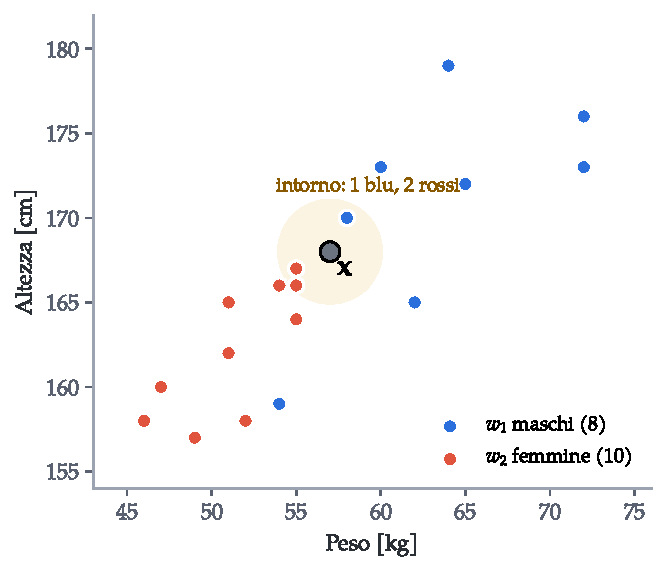
\includegraphics[width=\linewidth]{figs/conteggio.pdf}
\end{minipage}
\didascalia{Dati reali della slide 54; il pattern $\x=(57,\,168)$ ha nel cerchio 1 maschio e 2 femmine.}

\subsection{Il calcolo in quattro passi}
\begin{esempio}[Passo 1: prior]
Si contano gli esempi di ciascuna classe e si divide per il totale: $\;P(w_i)\approx n_i/n$.
\[
P(w_1)=\frac{8}{18}\approx0.44\qquad\qquad P(w_2)=\frac{10}{18}\approx0.56
\]
\end{esempio}
\begin{esempio}[Passo 2: densità condizionali]
Si contano i punti di ciascuna classe nel cerchio, in proporzione al \emph{totale della classe}:
\[
p(\x\,|\,w_1)\approx\frac{k_1}{n_1}=\frac18\qquad\qquad p(\x\,|\,w_2)\approx\frac{k_2}{n_2}=\frac{2}{10}=\frac15
\]
Si divide per $n_i$ e non per 18 perché è una probabilità \emph{condizionata alla classe}: l'universo è solo la classe $w_i$.
\end{esempio}
\begin{esempio}[Passo 3: densità assoluta]
\[
p(\x)=\frac18\cdot\frac{8}{18}+\frac15\cdot\frac{10}{18}=\frac1{18}+\frac2{18}=\frac3{18}=\frac16
\]
Lettura: 3 delle 18 persone cadono nel cerchio. La formula «complicata» conta i punti nel cerchio sul totale.
\end{esempio}
\begin{esempio}[Passo 4: posteriori e decisione]
\[
P(w_1\,|\,\x)=\frac{1/18}{1/6}=\frac13\qquad\qquad P(w_2\,|\,\x)=\frac{2/18}{1/6}=\frac23\qquad\Rightarrow\qquad \x\to w_2\ \text{(femmina)}
\]
Confidenza del 67\%. Per \emph{decidere} bastava confrontare $1/18$ e $2/18$.
\end{esempio}

\subsection{Il trucco nascosto: la posteriori è una proporzione}
Nel cerchio c'è 1 blu su 3 punti e $P(w_1|\x)=1/3$; ci sono 2 rossi su 3 e $P(w_2|\x)=2/3$. Non è un caso:
\begin{formulat}{Stima a conteggio}
$\displaystyle p(\x|w_i)\,P(w_i)=\frac{k_i}{n_i}\cdot\frac{n_i}{n}=\frac{k_i}{n}
\qquad\Longrightarrow\qquad
P(w_i\,|\,\x)=\frac{k_i/n}{k/n}=\frac{k_i}{k}$
\end{formulat}
dove $k$ è il numero totale di punti nel cerchio. Gli $n_i$ si semplificano e la regola diventa «guarda i vicini e scegli la classe più rappresentata».

\begin{mlbox}
È esattamente l'idea del \textbf{k-Nearest Neighbors (k-NN)}: il k-NN è un classificatore bayesiano «travestito», in cui le densità sono stimate in modo non parametrico.
\end{mlbox}

\subsection{Precisazione: $1/8$ non è davvero una densità}
\begin{tecnica}
Tecnicamente $1/8$ è una \emph{probabilità}: quella che un maschio cada nel cerchio. Per avere una vera densità si divide per l'area (il volume) $V$ del cerchio, come si divide una massa per un volume per ottenere la densità fisica:
\[
p(\x\,|\,w_i)\approx\frac{k_i}{n_i\,V}
\]
Il risultato del prof resta corretto perché $V$ è lo \textbf{stesso} per entrambe le classi e si semplifica nella formula di Bayes. Questa formula è il punto di partenza dell'approccio non parametrico (\emph{Parzen Window}).
\end{tecnica}

\subsection{Perché la stima è «grossolana»}
\begin{attenzione}[Limiti del metodo]
\begin{itemize}
  \item \textbf{Dipende dal raggio}: un cerchio più grande può ribaltare la decisione, uno più piccolo può essere vuoto ($0/0$).
  \item \textbf{Instabile con pochi dati}: con 1 e 2 punti, una persona in più cambia molto le stime.
  \item \textbf{Maledizione della dimensionalità}: con molte feature i cerchi restano quasi vuoti.
  \item Bisogna \textbf{conservare tutto il training set} e ricontare per ogni nuovo $\x$.
\end{itemize}
\end{attenzione}
\textbf{Effetto del prior.} Con classi equiprobabili: $P(w_2|\x)=0.2/(0.125+0.2)\approx0.62$ invece di $0.67$. Stessa decisione, confidenza un po' più bassa. Nella sezione 11 lo \emph{stesso} esempio è risolto con le gaussiane.

\begin{appunti}{— Sezione 4}
\pag{20} $d=2$ (peso, altezza); 18 esempi: 8 maschi ($w_1$, blu), 10 femmine ($w_2$, rosso). Il cerchio è l'intorno per stimare le densità.
\pag{21} Prior: $P(w_i)\approx n_i/n=8/18,\ 10/18$ (training set rappresentativo, altrimenti classi equiprobabili). Likelihood: $k_i/n_i=1/8,\ 1/5$. Densità vera: $k_i/(n_iV)$, ma $V$ si semplifica. $p(\x)=3/18=1/6$.
\pag{22} $P(w_1|\x)=1/3$, $P(w_2|\x)=2/3$ $\Rightarrow$ \textbf{femmina}. Scorciatoia: $P(w_i|\x)=k_i/k$ $\Rightarrow$ logica del k-NN. Prior uguali: $0.62$. Limiti: raggio, pochi dati, dimensionalità, memoria.
\end{appunti}

\sezione{5}{Parametrico vs non parametrico}{23–25}

Sezione breve ma di snodo: spiega \emph{perché} il resto della lezione prende la strada che prende.

\subsection{Il problema di fondo}
\begin{center}
\rowcolors{2}{chiaro}{white}
\begin{tabularx}{\linewidth}{l l Y}
\rowcolor{navy}\thd{Ingrediente} & \thd{Difficoltà} & \thd{Perché}\\
Prior $P(w_i)$ & \textcolor{verde}{\textbf{facile}} & pochi numeri: conteggi, oppure classi equiprobabili\\
Likelihood $p(\x|w_i)$ & \textcolor{rosso}{\textbf{difficile}} & è un'intera \emph{funzione} su tutto lo spazio, da ricostruire a partire da pochi punti\\
\end{tabularx}
\end{center}
\begin{intuizione}
Stimare un prior è come stimare «la percentuale di maschi»: un solo numero. Stimare $p(\x|\text{maschi})$ è come disegnare la mappa completa di «dove stanno i maschi» nel piano peso-altezza, con la densità in \emph{ogni} punto, avendo visto solo 8 persone. Per questo le densità condizionali sono note «solo in teoria».
\end{intuizione}

\subsection{Le due soluzioni}
\begin{tcbraster}[raster columns=2,raster equal height,raster column skip=10pt]
\begin{tcolorbox}[base,colback=blu!6,colbacktitle=blu,coltitle=white,borderline west={3pt}{0pt}{blu},title={Parametrico},top=13pt,unbreakable]
«Scommetto che i dati hanno una certa \textbf{forma}; devo solo trovare i pochi numeri che la descrivono.»
\begin{itemize}
  \item si \emph{assume} la famiglia: gaussiana (multinormale);
  \item si stimano solo i \textbf{parametri} $\mmu$ e $\SSigma$;
  \item poi i dati di training si possono buttare.
\end{itemize}
\end{tcolorbox}
\begin{tcolorbox}[base,colback=ambra!7,colbacktitle=ambra,coltitle=white,borderline west={3pt}{0pt}{ambra},title={Non parametrico},top=13pt,unbreakable]
«Non assumo nulla sulla forma: lascio che siano i \textbf{dati} a disegnarla.»
\begin{itemize}
  \item nessuna forma imposta;
  \item la densità si costruisce dai punti (\emph{Parzen Window}; il cerchio della sezione 4 ne è una versione grezza);
  \item bisogna conservare tutto il training set.
\end{itemize}
\end{tcolorbox}
\end{tcbraster}

\begin{attenzione}[Il nome inganna]
«Non parametrico» \textbf{non} vuol dire «senza parametri». Vuol dire che il numero di parametri \textbf{cresce con i dati}: in un k-NN i dati stessi sono i parametri. Un modello parametrico ha invece un numero di parametri \emph{fisso}, qualunque sia la dimensione del training set.
\end{attenzione}

\subsection{Quando usare quale}
Il parametrico si usa quando valgono \textbf{entrambe} le condizioni: (1) c'è una «ragionevole certezza (o \emph{speranza})» che la forma sia adeguata, e (2) il training set è troppo piccolo per una buona stima non parametrica. Il corsivo su \emph{speranza} è voluto: spesso è un'ipotesi di comodo, da verificare (sezione 12).

\begin{center}
\rowcolors{2}{chiaro}{white}
\begin{tabularx}{\linewidth}{l Y Y}
\rowcolor{navy} & \thd{Parametrico} & \thd{Non parametrico}\\
Ipotesi sulla forma & forte (es. gaussiana) & nessuna\\
N. parametri & fisso & cresce con i dati\\
Dati necessari & pochi & molti\\
Rischio principale & \textbf{underfitting} se la forma è sbagliata & \textbf{overfitting} se i dati sono pochi\\
Memoria / velocità & leggero, veloce & conserva tutto, lento in predizione\\
Esempi & Bayes con multinormali, Naive Bayes, regressione logistica & Parzen Window, k-NN, alberi di decisione\\
\end{tabularx}
\end{center}

\subsection{Gradi di libertà e overfitting}
\begin{tecnica}[Gradi di libertà]
Numero di parametri indipendenti che il modello può regolare per adattarsi ai dati: misurano la sua \textbf{flessibilità} (capacità espressiva).
\begin{itemize}
  \item gaussiana 1D: \textbf{2} parametri ($\mu,\sigma$);
  \item multinormale in $d$ dimensioni: $d+\frac{d(d+1)}{2}$ per classe, cioè \textbf{5} con $d=2$;
  \item non parametrico: il modello «ricorda» ogni punto, quindi la flessibilità cresce con $n$.
\end{itemize}
\end{tecnica}
\begin{intuizione}[Perché pochi gradi di libertà = meno overfitting]
Un modello molto flessibile, con pochi dati, ha «troppa libertà»: si piega attorno a ogni punto, compresi quelli anomali (\textbf{overfitting}: va benissimo sul training e male sui dati nuovi). Un modello rigido come la gaussiana, con i suoi 5 numeri, \emph{non può} inseguire ogni punto: è costretto a catturare la tendenza generale. Il prezzo: se la forma è sbagliata non si adatta neanche con tanti dati (\textbf{underfitting}).
\end{intuizione}

\fig[.98\linewidth]{param_nonparam.pdf}
\didascalia{Sinistra: dati gaussiani e pochi campioni, la gaussiana stimata è già buona mentre le finestre producono picchi. Destra: dati bimodali e molti campioni, la gaussiana è sbagliata qualunque sia $n$, le finestre ricostruiscono entrambe le gobbe.}

\begin{mlbox}[Il compromesso bias-varianza]
Parametrico = \emph{bias} alto (se la forma è sbagliata), varianza bassa. Non parametrico = bias basso, \emph{varianza} alta con pochi dati. L'obiettivo di tutto il ML, come dice la slide 25: imparare i pattern reali nei dati \emph{senza memorizzare il rumore}. Anche il non parametrico ha un parametro da scegliere bene: la larghezza $h$ della finestra.
\end{mlbox}

\begin{appunti}{— Sezione 5}
\pag{23} Prior facili; likelihood difficile (intera funzione). \textbf{Parametrico}: si assume la forma, si stimano $\mmu,\SSigma$. \textbf{Non parametrico}: densità dai punti (Parzen), si conserva il training set. «Non parametrico» = n. parametri che cresce con i dati.
\pag{25} Parametrico se forma plausibile \textbf{e} pochi dati. Gradi di libertà = flessibilità: 2 (gaussiana 1D), $d+d(d+1)/2$ (multinormale). Pochi gradi $\Rightarrow$ meno overfitting; forma sbagliata $\Rightarrow$ underfitting. Compromesso bias-varianza.
\end{appunti}

\sezione{6}{La normale univariata e la stima MLE}{26–30}

Inizia l'approccio parametrico. Si parte dal caso più semplice, una sola feature ($d=1$), per capire \emph{com'è fatta} la gaussiana e \emph{come si stimano} i suoi parametri dai dati.

\subsection{La distribuzione normale}
\begin{formulat}{Densità normale ($d=1$)}
$\displaystyle p(x)=\frac{1}{\sigma\sqrt{2\pi}}\;\exp\!\left[-\frac{(x-\mu)^2}{2\sigma^2}\right]$
\end{formulat}
\begin{intuizione}
È la classica «campana»: la maggior parte dei valori si concentra attorno a un centro e quelli estremi diventano sempre più rari. Bastano \textbf{due numeri}: $\mu$ (media) dice \emph{dove} sta la campana, $\sigma$ (deviazione standard) quanto è \emph{larga}; $\sigma^2$ è la varianza.
\end{intuizione}

\begin{center}
\rowcolors{2}{chiaro}{white}
\begin{tabularx}{\linewidth}{>{\centering\arraybackslash}m{3cm} Y}
\rowcolor{navy}\thd{Pezzo} & \thd{Significato}\\
$(x-\mu)$ & distanza di $x$ dal centro\\
$(x-\mu)^2/\sigma^2$ & distanza al quadrato \textbf{misurata in unità di $\sigma$}: essere a 10 dal centro è «tanto» se $\sigma=2$, «poco» se $\sigma=50$. Diventerà la distanza di Mahalanobis\\
$\exp(-\,\cdot/2)$ & trasforma la distanza in plausibilità: distanza 0 → massimo; distanza grande → quasi 0\\
$1/(\sigma\sqrt{2\pi})$ & normalizzazione: area totale $=1$. Se $\sigma$ cresce, la campana si allarga e deve \emph{abbassarsi}\\
\end{tabularx}
\end{center}

\fig[.8\linewidth]{gauss_regola.pdf}
\didascalia{Regola 68–95–99.7: oltre $3\sigma$ il contributo è trascurabile (la gaussiana però non tocca mai lo zero).}

\begin{attenzione}[Il N.B. della slide 26]
Questa $p(x)$ è la densità di \emph{una} gaussiana; nel classificatore diventerà una $p(x|w_i)$, la densità di una classe. Non va confusa con la $p(\x)$ al denominatore di Bayes, che è la \emph{miscela} $\sum_i p(\x|w_i)P(w_i)$ di tutte le classi.
\end{attenzione}

\subsection{L'idea della Massima Verosimiglianza (MLE)}
\begin{intuizione}
Abbiamo 10 numeri: $\{3,\,7,\,9,\,-2,\,15,\,54,\,-11,\,0,\,23,\,-8\}$ e assumiamo che vengano da una gaussiana. \emph{Quale}? Una campana centrata su 100 rende i dati quasi impossibili; una strettissima centrata su 9 spiega il 9 ma non il 54. C'è una campana che rende i dati osservati «\textbf{più probabili possibile}»: è la stima MLE.
\end{intuizione}
\begin{formulat}{Funzione di verosimiglianza (campioni indipendenti)}
$\displaystyle L(\mu,\sigma)=\prod_{i=1}^{n} p(x_i\,|\,\mu,\sigma)
\qquad\qquad (\hat\mu,\hat\sigma)=\argmax_{\mu,\sigma} L(\mu,\sigma)$
\end{formulat}
Cambio di prospettiva: prima $p(x|\mu,\sigma)$ fissava i parametri e guardava $x$; ora i \textbf{dati sono fissi} (osservati) e variano i \textbf{parametri}.

\begin{mlbox}[MLE e MAP: due argmax diversi]
MAP (sezione 2): $\argmax$ sulle \emph{classi} di $P(\text{classe}|\text{dati})$, usa il prior. MLE: $\argmax$ sui \emph{parametri} di $p(\text{dati}|\text{parametri})$, senza prior. Aggiungendo un prior sui parametri si ottiene la stima MAP dei parametri.
\end{mlbox}

\subsection{Da dove vengono le formule}
\begin{tecnica}[Derivazione in tre passi]
\textbf{1. Logaritmo.} Massimizzare $L$ equivale a massimizzare $\ln L$ (il log è crescente) e il prodotto diventa una somma; in pratica evita anche l'\emph{underflow} numerico:
\[
\ell(\mu,\sigma^2)=-\frac n2\ln(2\pi\sigma^2)-\frac1{2\sigma^2}\sum_{i=1}^{n}(x_i-\mu)^2
\]
\textbf{2.} $\dfrac{\partial\ell}{\partial\mu}=0\;\Rightarrow\;\sum_i(x_i-\mu)=0\;\Rightarrow\;\hat\mu=\dfrac1n\sum_i x_i$\qquad (media campionaria)\\[4pt]
\textbf{3.} $\dfrac{\partial\ell}{\partial\sigma^2}=0\;\Rightarrow\;\hat\sigma^2=\dfrac1n\sum_i (x_i-\hat\mu)^2$\qquad (varianza campionaria)
\end{tecnica}
Intuizione del passo 2: massimizzare la likelihood gaussiana equivale a \textbf{minimizzare la somma dei quadrati} delle distanze dal centro, come nei minimi quadrati.

\subsection{L'esempio numerico}
\begin{esempio}[Stima di $\mu$ e $\sigma$ con $n=10$]
\[
\hat\mu=\frac{3+7+9-2+15+54-11+0+23-8}{10}=\frac{90}{10}=9
\]
\begin{center}\small
\begin{tabular}{l*{10}{c}}
\toprule
$x_i$ & 3 & 7 & 9 & $-2$ & 15 & \textcolor{rosso}{\textbf{54}} & $-11$ & 0 & 23 & $-8$\\
$x_i-9$ & $-6$ & $-2$ & 0 & $-11$ & 6 & \textcolor{rosso}{\textbf{45}} & $-20$ & $-9$ & 14 & $-17$\\
$(x_i-9)^2$ & 36 & 4 & 0 & 121 & 36 & \textcolor{rosso}{\textbf{2025}} & 400 & 81 & 196 & 289\\
\bottomrule
\end{tabular}
\end{center}
\[
\hat\sigma^2=\frac{3188}{10}=318.8\qquad\qquad \hat\sigma=\sqrt{318.8}\approx17.855
\]
(Nella slide 28 c'è un «$^2$» in più dopo l'ultima parentesi del numeratore: è un refuso, il risultato è corretto.)
\end{esempio}

\fig[.98\linewidth]{mle1d.pdf}
\didascalia{Sinistra: la gaussiana stimata e la densità nel punto 25. Destra: la log-verosimiglianza in funzione di $\mu$ ha il massimo proprio nella media campionaria.}

\begin{attenzione}[Due osservazioni importanti]
\textbf{a) L'outlier domina.} Il valore 54 contribuisce 2025 su 3188, cioè il \textbf{64\%} della varianza. Togliendolo: $\hat\mu=4$, $\hat\sigma\approx10.2$. Il MLE gaussiano è sensibile agli outlier perché eleva le distanze al quadrato.

\textbf{b) $n$ o $n-1$?} La MLE divide per $n$ ed è leggermente \emph{distorta} (sottostima). Dividendo per $n-1$ (correzione di Bessel) si ha la stima corretta: $3188/9\approx354.2$. La differenza conta solo con pochi dati. Il prof usa $1/n$, coerente con la MLE.
\end{attenzione}

\subsection{Densità $\neq$ probabilità}
\begin{formula}
$\displaystyle p(25)=\frac{1}{17.855\sqrt{2\pi}}\;e^{-\frac{(25-9)^2}{2\cdot318.8}}=\frac{1}{44.7559}\,e^{-0.4015}\approx0.01495$
\end{formula}
\begin{intuizione}
$p(25)$ \textbf{non} è «la probabilità di osservare esattamente 25»: nel continuo quella è 0. È una \emph{concentrazione} di probabilità attorno a 25. Per avere una probabilità si moltiplica per la larghezza di un intervallo:
\[
P(x\le X\le x+dx)\approx p(x)\,dx
\]
Come la densità di un materiale (kg/m$^3$) non è una massa finché non la si moltiplica per un volume.
\end{intuizione}
\begin{esempio}[Verifica numerica]
La probabilità esatta dell'intervallo $[24.5,\,25.5]$ (largo 1) vale $0.014954$, praticamente uguale a $p(25)\cdot1=0.014955$. Controllo di sanità: in $\hat\mu\pm2\hat\sigma=[-26.7,\,44.7]$ cadono 9 valori su 10; resta fuori solo il 54.
\end{esempio}
Una densità \textbf{può superare 1}: con $\sigma=0.1$ il picco vale circa $3.99$. Conta solo che l'area totale sia 1. Nella formula di Bayes il $dx$ si semplifica e la posteriori resta una vera probabilità.

\begin{appunti}{— Sezione 6}
\pag{26} $\mu$ = posizione, $\sigma$ = larghezza; $(x-\mu)^2/\sigma^2$ = distanza in unità di $\sigma$. $1/(\sigma\sqrt{2\pi})$: area 1. 68/95/99.7\% in $\pm1,2,3\sigma$. Questa $p(x)$ diventerà $p(x|w_i)$, $\neq$ evidence.
\pag{27} MLE: parametri che rendono i dati più verosimili. $L=\prod_i p(x_i|\mu,\sigma)$; dati fissi, parametri variabili; si massimizza $\ln L$. MLE (parametri, nessun prior) vs MAP (classi, con prior).
\pag{28} $\hat\mu=\bar x=9$; $\hat\sigma^2=318.8$; $\hat\sigma\approx17.855$. Outlier 54 = 64\% della varianza. MLE divide per $n$ (distorta); $n-1$: 354.2. Refuso: «$^2$» finale.
\pag{29–30} $p(25)\approx0.01495$ è una densità; $P([x,x+dx])\approx p(x)dx$; densità $>1$ possibile; in Bayes il $dx$ si semplifica.
\end{appunti}

\sezione{7}{Richiami di algebra lineare}{32–39}

Queste slide sono un attrezzo per la sezione 8: la gaussiana in $d$ dimensioni contiene una \textbf{matrice} (la covarianza $\SSigma$), la sua \textbf{inversa} $\SSigma^{-1}$ e il suo \textbf{determinante} $|\SSigma|$. Autovalori e autovettori spiegano la \emph{forma} della distribuzione.

\subsection{La matrice di covarianza}
\begin{intuizione}
In 1D la varianza dice quanto si sparpagliano i dati. Con più feature non basta: serve sapere anche \emph{come variano insieme}. Se una persona pesa di più, tende a essere più alta? La matrice di covarianza raccoglie tutte queste informazioni.
\end{intuizione}
\begin{tecnica}
\[
\sigma^{ij}=E\big[(x^i-\mu^i)(x^j-\mu^j)\big]
\qquad\qquad
\SSigma=\begin{pmatrix}\sigma^{11}&\sigma^{12}\\\sigma^{21}&\sigma^{22}\end{pmatrix}=\begin{pmatrix}\mathrm{var(peso)}&\mathrm{cov(peso,alt.)}\\\mathrm{cov(alt.,peso)}&\mathrm{var(altezza)}\end{pmatrix}
\]
\begin{itemize}
  \item \textbf{Diagonale} $\sigma^{ii}$: varianza della singola feature.
  \item \textbf{Fuori diagonale} $\sigma^{ij}$: $>0$ crescono insieme; $<0$ in verso opposto; $=0$ nessuna relazione lineare.
  \item \textbf{Simmetrica}: $\sigma^{ij}=\sigma^{ji}$, quindi $\SSigma=\SSigma\T$.
  \item \textbf{Definita positiva}: tutti gli autovalori $>0$, cioè la nuvola ha «spessore» in ogni direzione $\Rightarrow\ \det\SSigma>0\Rightarrow$ invertibile.
\end{itemize}
\end{tecnica}
\begin{attenzione}[«Sempre definita positiva»: vero in teoria, non sempre in pratica]
Una covarianza \emph{stimata} dai dati è in generale solo \textbf{semidefinita} (autovalori $\ge0$) e può essere \textbf{singolare}:
\begin{itemize}
  \item se una feature è combinazione lineare di altre (peso in kg e in libbre insieme);
  \item se ci sono meno campioni che dimensioni ($n\le d$).
\end{itemize}
Rimedio standard (\emph{regolarizzazione}): si aggiunge un piccolo valore sulla diagonale, $\SSigma+\varepsilon I$.
\end{attenzione}

\subsection{Trasposta, simmetrica, coniugata}
\begin{itemize}
  \item \textbf{Trasposta} $A\T$: si scambiano righe e colonne; un vettore colonna diventa riga (l'apice $\mathsf{t}$ in $(\x-\mmu)\T$).
  \item \textbf{Simmetrica}: $A=A\T$ (quadrata, speculare rispetto alla diagonale).
  \item \textbf{Trasposta coniugata} $A^*$: per matrici complesse. Per matrici reali $A^*=A\T$: per noi è irrilevante.
\end{itemize}

\subsection{Inversa, aggiunta, cofattori}
\begin{intuizione}
L'inversa $A^{-1}$ «annulla» $A$: $AA^{-1}=I$, come $4\times\frac14=1$. Esiste solo se $\det A\neq0$, come non esiste $1/0$.
\end{intuizione}
\begin{tecnica}[La ricetta della slide 33]
\begin{enumerate}
  \item \textbf{Minore} $M_{ij}$: determinante della matrice ottenuta eliminando riga $i$ e colonna $j$.
  \item \textbf{Cofattore}: $C_{ij}=(-1)^{i+j}M_{ij}$ (segni a scacchiera $+,-,+,\dots$).
  \item \textbf{Aggiunta classica}: $\operatorname{adj}(A)$ = \emph{trasposta} della matrice dei cofattori.
  \item \textbf{Inversa}: $A^{-1}=\operatorname{adj}(A)/\det A$.
\end{enumerate}
\end{tecnica}
\begin{formulat}{Inversa di una matrice $2\times2$}
$\displaystyle \begin{pmatrix}a&b\\c&d\end{pmatrix}^{-1}=\frac{1}{ad-bc}\begin{pmatrix}d&-b\\-c&a\end{pmatrix}$
\qquad «scambia la diagonale, cambia segno al resto, dividi per il determinante»
\end{formulat}
\begin{esempio}[$A=\begin{pmatrix}4&2\\2&3\end{pmatrix}$, simmetrica come una covarianza]
$\det A=4\cdot3-2\cdot2=8$; cofattori $C_{11}=3,\ C_{12}=-2,\ C_{21}=-2,\ C_{22}=4$;
\[
A^{-1}=\frac18\begin{pmatrix}3&-2\\-2&4\end{pmatrix}
\qquad\text{verifica: }\ \frac{4\cdot3+2\cdot(-2)}{8}=1\ \checkmark
\]
\end{esempio}
\begin{attenzione}[Trappola di nomenclatura]
In italiano «aggiunta» può indicare l'\textbf{aggiunta classica} $\operatorname{adj}(A)$ (\emph{adjugate}, quella dei cofattori) o la \textbf{trasposta coniugata} $A^*$ (\emph{adjoint}). Coincidono solo se $A^*A=\det(A)\,I$: è il senso dell'ultimo punto della slide. In pratica nessuno inverte con i cofattori oltre $3\times3$: le librerie usano metodi numerici (LU, Cholesky).
\end{attenzione}

\subsection{Autovalori e autovettori}
\begin{formulat}{Definizione}
$\displaystyle A\vv=\lambda\vv,\qquad \vv\neq\mathbf{0}\qquad\qquad \det(A-\lambda I)=0\ \ \text{(equazione caratteristica)}$
\end{formulat}
\begin{intuizione}[Interpretazione geometrica (slide 36)]
Una matrice è una \textbf{trasformazione} del piano: prende ogni vettore e lo sposta altrove, in genere ruotandolo e stirandolo. Esistono però direzioni speciali che la trasformazione \textbf{non ruota}: le stira o le accorcia soltanto. Sono gli \key{autovettori}; il fattore di stiramento è l'\key{autovalore} ($\lambda>1$ allunga, $0<\lambda<1$ accorcia, $\lambda<0$ inverte, $\lambda=0$ schiaccia).
\end{intuizione}
\fig[.9\linewidth]{autovettori.pdf}
\didascalia{Il cerchio unitario diventa un'ellisse; gli autovettori sono gli assi dell'ellisse e gli autovalori le lunghezze dei semiassi. A sinistra, $\mathbf{w}=(1,1)$ cambia direzione: non è un autovettore.}

\begin{esempio}[Le slide 36–39 e un caso meno banale]
$A=\mathrm{diag}(2,1)$: $\ \vv=(1,0)\to A\vv=(2,0)=2\vv$, autovettore con $\lambda=2$; l'asse $y$ resta identico ($\lambda=1$). Equazione caratteristica: $(2-\lambda)(1-\lambda)=0$. Per una matrice diagonale gli autovalori sono gli elementi della diagonale.

$A=\begin{pmatrix}4&2\\2&3\end{pmatrix}$: $\ (4-\lambda)(3-\lambda)-4=\lambda^2-7\lambda+8=0\;\Rightarrow\;\lambda=\frac{7\pm\sqrt{17}}2\approx5.56,\ 1.44$. Entrambi positivi: definita positiva. Verifica: $\lambda_1\lambda_2\approx8=\det A$.
\end{esempio}
Se $\vv$ è autovettore lo è anche $\alpha\vv$ ($\alpha\neq0$, slide 35): conta la direzione, non la lunghezza. Per convenzione si normalizza a lunghezza 1.

\subsection{Il ponte verso la gaussiana multivariata}
\begin{center}
\rowcolors{2}{chiaro}{white}
\begin{tabularx}{\linewidth}{>{\raggedright\arraybackslash}p{5.6cm} Y}
\rowcolor{navy}\thd{Proprietà ($\SSigma$ simmetrica)} & \thd{Conseguenza per la multinormale}\\
autovalori reali, autovettori perpendicolari & sistema di assi «naturale» per i dati\\
autovettori di $\SSigma$ & direzioni degli \textbf{assi dell'ellisse} (orientamento)\\
autovalori di $\SSigma$ & \textbf{varianze lungo gli assi} ($\sqrt\lambda$ = semiasse)\\
$\det\SSigma=\lambda_1\lambda_2\cdots\lambda_d$ & «volume» della nuvola: il $|\SSigma|$ della normalizzazione\\
$\SSigma^{-1}$: stessi autovettori, autovalori $1/\lambda$ & in Mahalanobis «accorcia» le direzioni molto sparse\\
tutti $\lambda>0\iff$ invertibile & senza, la gaussiana non si può scrivere\\
\end{tabularx}
\end{center}
\begin{mlbox}
Calcolare gli autovettori della covarianza dei dati è esattamente la \textbf{PCA} (\emph{Principal Component Analysis}): l'autovettore con l'autovalore più grande è la direzione di massima variabilità.
\end{mlbox}

\begin{appunti}{— Sezione 7}
\pag{32} $\SSigma$: diagonale = varianze, fuori diagonale = covarianze ($>0,<0,=0$). Simmetrica. Definita positiva $\Rightarrow$ invertibile. Stimata può essere \textbf{singolare} ($n\le d$, feature dipendenti): $\SSigma+\varepsilon I$.
\pag{33} Minore → cofattore $(-1)^{i+j}M_{ij}$ → trasposta = adj → $A^{-1}=\operatorname{adj}A/\det A$. $2\times2$: $\frac1{ad-bc}\begin{psmallmatrix}d&-b\\-c&a\end{psmallmatrix}$. «Aggiunta» ambigua (adj vs $A^*$).
\pag{34–38} $A\vv=\lambda\vv$: direzione non ruotata, $\lambda$ = stiramento. Anche $\alpha\vv$ è autovettore.
\pag{39} $\det(A-\lambda I)=0$. Esempio $\begin{psmallmatrix}4&2\\2&3\end{psmallmatrix}$: $\lambda\approx5.56,\ 1.44$.
\textbf{Ponte:} autovettori = assi dell'ellisse; autovalori = varianze lungo gli assi; $\det$ = volume; = PCA.
\end{appunti}

\sezione{8}{Normale multivariata e distanza di Mahalanobis}{31, 40–43}

Qui tutti i pezzi della sezione 7 si incastrano: la campana della sezione 6 viene generalizzata a $d$ feature.

\subsection{Notazione}
\begin{itemize}
  \item $\x_i$: pattern $i$-esimo del training set (\textbf{vettore}, indice in basso);
  \item $x_i^j$: componente $j$-esima del pattern $i$-esimo (\textbf{scalare}, indice in alto). Attenzione: l'apice è un indice, non una potenza.
  \item I vettori sono \emph{colonne}; l'apice $\mathsf{t}$ li trasforma in righe.
\end{itemize}

\subsection{La formula}
\begin{formulat}{Densità multinormale ($d>1$)}
$\displaystyle p(\x)=\frac{1}{(2\pi)^{d/2}\,|\SSigma|^{1/2}}\;\exp\!\left[-\frac12\,(\x-\mmu)\T\,\SSigma^{-1}\,(\x-\mmu)\right]$
\end{formulat}
dove $\mmu=[\mu^1,\dots,\mu^d]\T$ è il \key{vettore medio} e $\SSigma=[\sigma^{ij}]$ la \key{matrice di covarianza} $d\times d$.

\begin{intuizione}[Confronto pezzo per pezzo con il caso 1D]
\begin{center}
\begin{tabular}{lcc}
\toprule
& \textbf{1D} & \textbf{$d$ dimensioni}\\
\midrule
centro & $\mu$ & $\mmu$\\
«larghezza» & $\sigma^2$ & $\SSigma$\\
distanza al quadrato & $(x-\mu)^2/\sigma^2$ & $(\x-\mmu)\T\SSigma^{-1}(\x-\mmu)$\\
normalizzazione & $\sigma\sqrt{2\pi}$ & $(2\pi)^{d/2}|\SSigma|^{1/2}$\\
\bottomrule
\end{tabular}
\end{center}
Dividere per $\sigma^2$ diventa moltiplicare per $\SSigma^{-1}$; la $\sigma$ della normalizzazione diventa $|\SSigma|^{1/2}$, il «volume» della nuvola.
\end{intuizione}
\begin{tecnica}[Le dimensioni tornano]
$(\x-\mmu)\T$ è $1\times d$, $\SSigma^{-1}$ è $d\times d$, $(\x-\mmu)$ è $d\times1$: il prodotto è $1\times1$, cioè un \textbf{numero}. L'esponente è uno scalare, come deve essere.
\end{tecnica}

\subsection{Quanti parametri?}
$\SSigma$ è simmetrica, quindi basta conoscere la diagonale e metà degli elementi restanti: $\dfrac{d(d+1)}{2}$ parametri, più i $d$ della media.
\begin{center}
\rowcolors{2}{chiaro}{white}
\begin{tabular}{cccc}
\rowcolor{navy}\thd{$d$} & \thd{media} & \thd{covarianza piena} & \thd{covarianza diagonale}\\
2 & 2 & 3 & 2\\
10 & 10 & 55 & 10\\
100 & 100 & 5050 & 100\\
\end{tabular}
\end{center}
Con molte feature la covarianza piena richiede moltissimi dati per essere stimata bene (e per essere invertibile, sezione 7): è uno dei motivi del successo del Naive Bayes.

\subsection{Varianze e covarianze}
Gli elementi diagonali $\sigma^{ii}=(\sigma^i)^2$ sono le varianze delle singole feature; quelli fuori diagonale le covarianze:
\begin{itemize}
  \item $x^i,x^j$ statisticamente indipendenti $\Rightarrow\sigma^{ij}=0$;
  \item correlate positivamente $\Rightarrow\sigma^{ij}>0$ (quando cresce una cresce l'altra);
  \item correlate negativamente $\Rightarrow\sigma^{ij}<0$.
\end{itemize}
\begin{attenzione}[L'implicazione vale in un solo verso]
Indipendenza $\Rightarrow$ covarianza nulla, ma in generale \textbf{non} il contrario: la covarianza misura solo legami \emph{lineari} ($x$ e $x^2$ con $x$ simmetrica attorno a 0 hanno covarianza nulla ma sono dipendenti). Per la gaussiana multivariata, invece, covarianza nulla e indipendenza coincidono.
\end{attenzione}

\subsection{La forma: ellissi a densità costante}
Per $d=2$ le curve di livello della densità sono \textbf{ellissi} concentriche: i luoghi dei punti a densità costante.
\fig[.98\linewidth]{multinormali.pdf}
\didascalia{Stessa media, tre covarianze diverse. In arancione gli assi dell'ellisse, paralleli agli autovettori di $\SSigma$.}
\begin{tecnica}[Chi controlla cosa (slide 41–42)]
\begin{itemize}
  \item $\mmu=[\mu^1,\mu^2]$: posizione del \textbf{centro};
  \item $\sigma^{11},\sigma^{22}$: \textbf{allungamento} lungo i due assi;
  \item $\sigma^{12}=\sigma^{21}$: \textbf{rotazione} dell'ellisse rispetto agli assi cartesiani;
  \item gli assi dell'ellisse sono paralleli agli \textbf{autovettori} di $\SSigma$; le varianze lungo gli assi principali sono gli \textbf{autovalori}.
\end{itemize}
\end{tecnica}

\subsection{Covarianza diagonale e Naive Bayes}
Se $\sigma^{12}=0$ (matrice diagonale) gli assi dell'ellisse sono paralleli agli assi cartesiani e la multinormale si spezza in un \textbf{prodotto di $d$ normali 1D}:
\begin{formulat}{Covarianza diagonale}
$\displaystyle p(\x)=\prod_{j=1}^{d}\frac{1}{\sigma^j\sqrt{2\pi}}\exp\!\left[-\frac{(x^j-\mu^j)^2}{2(\sigma^j)^2}\right]$
\end{formulat}
\begin{mlbox}[Naive Bayes]
Il classificatore \textbf{Naive Bayes} assume che le feature siano indipendenti \emph{data la classe}: $p(\x|w_i)=\prod_j p(x^j|w_i)$. Con gaussiane è esattamente il caso diagonale: $2d$ parametri per classe invece di $d+d(d+1)/2$, nessuna matrice da invertire, stime stabili anche con pochi dati. L'ipotesi è quasi sempre falsa («naive», ingenua), eppure funziona bene su molti dataset, in particolare per la classificazione di testi: per questo è tra i classificatori più popolari.
\end{mlbox}

\subsection{La distanza di Mahalanobis}
\begin{formulat}{Distanza di Mahalanobis}
$\displaystyle r^2=(\x-\mmu)\T\,\SSigma^{-1}\,(\x-\mmu)\qquad\Longrightarrow\qquad p(\x)=\frac{1}{(2\pi)^{d/2}|\SSigma|^{1/2}}\,e^{-r^2/2}$
\end{formulat}
\begin{intuizione}
La densità dipende da $\x$ solo attraverso $r$: le ellissi a densità costante sono esattamente i luoghi a \textbf{distanza di Mahalanobis costante} ($r=1,2,3,\dots$). È la generalizzazione di «quante $\sigma$ dista dal centro?». Rispetto alla distanza euclidea, Mahalanobis \textbf{pesa} ogni direzione in base a quanto i dati variano lungo di essa e tiene conto della \textbf{correlazione}: un passo lungo la direzione in cui la nuvola è allungata conta poco, uno nella direzione stretta conta molto.
\end{intuizione}
\begin{minipage}[c]{.5\linewidth}
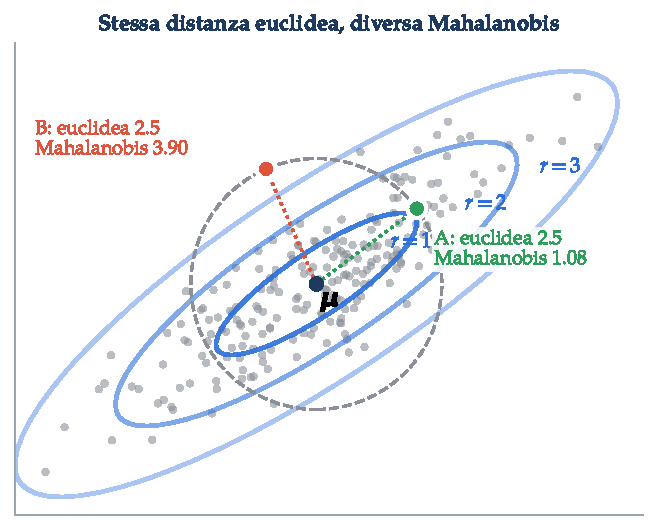
\includegraphics[width=\linewidth]{figs/mahalanobis.pdf}
\end{minipage}\hfill
\begin{minipage}[c]{.47\linewidth}\raggedright
\begin{esempio}[Stessa distanza euclidea]
I punti A e B distano entrambi 2.5 dal centro (cerchio tratteggiato), ma:
\begin{itemize}
  \item A sta lungo l'asse lungo della nuvola: $r\approx1.08$, è un punto \emph{tipico};
  \item B va «contro» la correlazione: $r\approx3.90$, è quasi un \emph{outlier}.
\end{itemize}
La distanza euclidea non vede la differenza; Mahalanobis sì.
\end{esempio}
\end{minipage}

\begin{tecnica}[Casi particolari]
\begin{itemize}
  \item $\SSigma=I$: $r^2=\|\x-\mmu\|^2$, Mahalanobis \textbf{coincide} con l'euclidea.
  \item $\SSigma$ diagonale: $r^2=\sum_j (x^j-\mu^j)^2/(\sigma^j)^2$, euclidea sulle feature \emph{standardizzate}.
  \item Se $\x$ è davvero gaussiano, $r^2$ segue una distribuzione $\chi^2$ con $d$ gradi di libertà: utile per riconoscere gli outlier.
\end{itemize}
\end{tecnica}
\begin{mlbox}
Mahalanobis si usa al posto dell'euclidea in k-NN e clustering quando le feature hanno scale diverse o sono correlate, e nel rilevamento di anomalie. Standardizzare le feature (z-score) prima di un k-NN è la versione «diagonale» della stessa idea.
\end{mlbox}

\begin{appunti}{— Sezione 8}
\pag{31} Pedice = pattern, apice = componente. $p(\x)=\frac{1}{(2\pi)^{d/2}|\SSigma|^{1/2}}\exp[-\frac12(\x-\mmu)\T\SSigma^{-1}(\x-\mmu)]$. Analogia 1D: $\sigma^2\to\SSigma$, $1/\sigma^2\to\SSigma^{-1}$, $\sigma\to|\SSigma|^{1/2}$. L'esponente è uno scalare.
\pag{40} Colonne, $\mathsf{t}$ = riga. Parametri di $\SSigma$: $d(d+1)/2$ (+ $d$ per $\mmu$). $\sigma^{ii}$ varianze; $\sigma^{ij}$ covarianze. Indipendenza $\Rightarrow\sigma^{ij}=0$ (il contrario vale per la gaussiana, non in generale).
\pag{41} $d=2$: ellissi = densità costante. $\mmu$ = centro; $\sigma^{11},\sigma^{22}$ = allungamento.
\pag{42} $\sigma^{12}$ = rotazione. $=0$: assi paralleli, prodotto di $d$ normali 1D = \textbf{Naive Bayes} ($2d$ parametri). Assi ∥ autovettori; varianze = autovalori. Naive Bayes funziona bene anche se l'ipotesi è falsa.
\pag{43} $r^2=(\x-\mmu)\T\SSigma^{-1}(\x-\mmu)$: le ellissi sono $r$ costante. Pesa per varianza e correlazione. $\SSigma=I$ → euclidea. Esempio: stessa euclidea 2.5, Mahalanobis 1.08 vs 3.90.
\end{appunti}

\sezione{9}{Stima MLE in due dimensioni: esempio svolto}{44–49}

Stesso principio della sezione 6 (massima verosimiglianza), ora con vettori e matrici.

\subsection{I dati}
Training set di $n=5$ pattern bidimensionali:
\[
\left\{\,[3,\,7]\T,\ [4.5,\,12]\T,\ [13,\,7.2]\T,\ [1,\,4]\T,\ [23,\,15.8]\T\,\right\}
\]

\subsection{Le formule MLE}
\begin{formulat}{Stime di massima verosimiglianza}
$\displaystyle \mmu=\frac1n\sum_{i=1}^{n}\x_i
\qquad\qquad
\SSigma=\frac1n\sum_{i=1}^{n}(\x_i-\mmu)(\x_i-\mmu)\T$
\end{formulat}
\begin{intuizione}
La media vettoriale è la media \emph{componente per componente}. La covarianza è una somma di matrici: ogni pattern contribuisce con il prodotto «colonna per riga» del suo scarto dalla media, una matrice $2\times2$ che dice in quale direzione quel punto si allontana dal centro. Elemento per elemento:
\[
\sigma^{ij}=\frac1n\sum_{k=1}^{n}(x_k^i-\mu^i)(x_k^j-\mu^j)
\]
\end{intuizione}

\subsection{Il vettore medio}
\begin{esempio}
\[
\mmu=\begin{bmatrix}\dfrac{3+4.5+13+1+23}{5}\\[8pt]\dfrac{7+12+7.2+4+15.8}{5}\end{bmatrix}=\begin{bmatrix}8.9\\9.2\end{bmatrix}
\]
\end{esempio}

\subsection{La matrice di covarianza}
\begin{esempio}[Prodotti «colonna per riga» degli scarti]
\begin{center}\small
\rowcolors{2}{chiaro}{white}
\begin{tabular}{ccc}
\rowcolor{navy}\thd{$\x_i$} & \thd{$\x_i-\mmu$} & \thd{$(\x_i-\mmu)(\x_i-\mmu)\T$}\\
$[3,\,7]$ & $[-5.9,\,-2.2]$ & $\begin{psmallmatrix}34.81&12.98\\12.98&4.84\end{psmallmatrix}$\\[3pt]
$[4.5,\,12]$ & $[-4.4,\,2.8]$ & $\begin{psmallmatrix}19.36&-12.32\\-12.32&7.84\end{psmallmatrix}$\\[3pt]
$[13,\,7.2]$ & $[4.1,\,-2.0]$ & $\begin{psmallmatrix}16.81&-8.20\\-8.20&4.00\end{psmallmatrix}$\\[3pt]
$[1,\,4]$ & $[-7.9,\,-5.2]$ & $\begin{psmallmatrix}62.41&41.08\\41.08&27.04\end{psmallmatrix}$\\[3pt]
$[23,\,15.8]$ & $[14.1,\,6.6]$ & $\begin{psmallmatrix}198.81&93.06\\93.06&43.56\end{psmallmatrix}$\\
\end{tabular}
\end{center}
Sommando le cinque matrici e dividendo per 5:
\[
\SSigma=\begin{bmatrix}\sigma^{11}&\sigma^{12}\\\sigma^{21}&\sigma^{22}\end{bmatrix}=\begin{bmatrix}66.44&25.32\\25.32&17.456\end{bmatrix}
\]
Per esempio $\sigma^{11}=(34.81+19.36+16.81+62.41+198.81)/5=332.2/5=66.44$.
\end{esempio}
\textbf{Lettura:} $\sigma^{12}>0$, quindi le due feature crescono insieme e l'ellisse è inclinata verso l'alto a destra. La varianza lungo $x^1$ (66.4) è molto maggiore di quella lungo $x^2$ (17.5): l'ellisse è allungata in orizzontale.

\subsection{Determinante e inversa}
\begin{esempio}
\[
|\SSigma|=66.44\cdot17.456-25.32^2=1159.78-641.10=518.674
\]
\[
\SSigma^{-1}=\frac{1}{518.674}\begin{bmatrix}17.456&-25.32\\-25.32&66.44\end{bmatrix}=\begin{bmatrix}0.0337&-0.0488\\-0.0488&0.1281\end{bmatrix}
\]
È la formula $2\times2$ della sezione 7: si scambiano gli elementi della diagonale, si cambia segno agli altri, si divide per il determinante.
\end{esempio}
\begin{tecnica}[In più: autovalori di questa $\SSigma$]
$\lambda_1\approx77.18,\ \lambda_2\approx6.72$. Verifiche: $\lambda_1+\lambda_2=83.90=66.44+17.456$ (traccia) e $\lambda_1\lambda_2\approx518.67=|\SSigma|$. L'asse principale punta a circa $23^\circ$ (direzione $\approx(0.92,\,0.39)$): l'ellisse è lunga $\sqrt{77.18}\approx8.8$ e larga $\sqrt{6.72}\approx2.6$ (in unità di $r=1$).
\end{tecnica}

\fig[.98\linewidth]{stima2d.pdf}
\didascalia{La gaussiana stimata vista dall'alto (curve di livello, con gli autovettori scalati per $2\sqrt{\lambda}$) e di lato (la campana bidimensionale). Corrisponde alla slide 49.}

\begin{attenzione}
\begin{itemize}
  \item Come in 1D, la MLE divide per $n$; con $n-1$ si otterrebbe $\begin{psmallmatrix}83.05&31.65\\31.65&21.82\end{psmallmatrix}$. Con soli 5 punti la differenza è grande (25\%).
  \item Con 5 punti in 2D la stima è molto incerta: il punto $[23,\,15.8]$ da solo pesa il 60\% di $\sigma^{11}$. Servono $n>d$ per l'invertibilità e molti più punti per una stima affidabile.
\end{itemize}
\end{attenzione}
\begin{mlbox}[Calcolo incrementale]
Vale l'identità $\SSigma=\frac1n\sum_i\x_i\x_i\T-\mmu\mmu\T$: basta tenere le somme $\sum_i\x_i$ e $\sum_i\x_i\x_i\T$ e aggiornarle a ogni nuovo esempio, senza conservare i dati. È la proprietà «incrementale» della sezione 3.
\end{mlbox}

\begin{appunti}{— Sezione 9}
\pag{44} 5 pattern 2D; stima MLE di vettore medio e covarianza.
\pag{45} $\mmu=\frac1n\sum_i\x_i=[8.9,\ 9.2]\T$ (media componente per componente).
\pag{46} $\SSigma=\frac1n\sum_i(\x_i-\mmu)(\x_i-\mmu)\T$: somma di matrici colonna $\times$ riga; $\sigma^{ij}=\frac1n\sum_k(x_k^i-\mu^i)(x_k^j-\mu^j)$.
\pag{47} $\SSigma=\begin{psmallmatrix}66.44&25.32\\25.32&17.456\end{psmallmatrix}$; $|\SSigma|=518.674$; $\SSigma^{-1}=\begin{psmallmatrix}0.0337&-0.0488\\-0.0488&0.1281\end{psmallmatrix}$. $\sigma^{12}>0$: ellisse inclinata.
\pag{48} Inversa $2\times2$: $\frac1{ad-bc}\begin{psmallmatrix}d&-b\\-c&a\end{psmallmatrix}$.
\pag{49} Autovalori $\approx77.2,\ 6.7$; asse principale a $\approx23^\circ$. Con $n-1$: stime più grandi del 25\%. $\SSigma=\frac1n\sum\x\x\T-\mmu\mmu\T$ (incrementale).
\end{appunti}

\sezione{10}{Bayes con multinormali e superfici decisionali}{50–53}

Ora ogni classe ha la sua gaussiana $p(\x|w_i)$, con i propri $\mmu_i$ e $\SSigma_i$. La regola resta quella della sezione 2: in ogni punto vince la classe con $p(\x|w_i)P(w_i)$ più alto. Cambia la \emph{forma} del confine.

\subsection{Regioni e superfici decisionali}
\begin{intuizione}
Immagina due «montagne» sopra il piano delle feature, alte $p(\x|w_1)P(w_1)$ e $p(\x|w_2)P(w_2)$ (slide 50). Ogni punto del piano appartiene alla classe la cui montagna è più alta lì sopra. Il \key{confine di decisione} (\emph{decision boundary} o \emph{decision surface}) è la linea dove le due montagne hanno la stessa altezza: lì la classificazione è \textbf{ambigua}.
\end{intuizione}
Lo spazio viene suddiviso in regioni $\Re_i$ che \textbf{non devono essere connesse}: nell'esempio della slide 50, $\Re_2$ è formata da due pezzi separati e il confine è composto da due iperboli.

\begin{minipage}[c]{.5\linewidth}
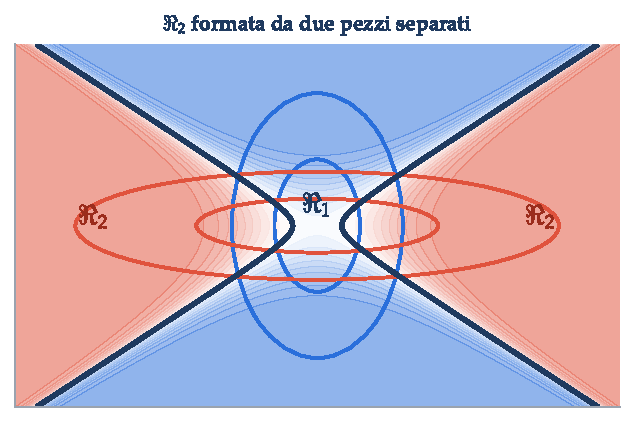
\includegraphics[width=\linewidth]{figs/regioni_disgiunte.pdf}
\end{minipage}\hfill
\begin{minipage}[c]{.46\linewidth}\raggedright
\small Due classi con la stessa media: la blu è più estesa in verticale, la rossa è lunga in orizzontale ma sottile. Sopra e sotto vince la blu, ai due lati la rossa. Il confine è formato da due \textbf{iperboli} e $\Re_2$ è spezzata in due regioni disgiunte, come nella slide 50.
\end{minipage}

\subsection{Le funzioni discriminanti}
\begin{tecnica}[Passare ai logaritmi]
Il logaritmo è crescente e non cambia l'argmax, quindi si può confrontare
\[
g_i(\x)=\ln p(\x|w_i)+\ln P(w_i)=-\frac12(\x-\mmu_i)\T\SSigma_i^{-1}(\x-\mmu_i)-\frac12\ln|\SSigma_i|-\frac d2\ln2\pi+\ln P(w_i)
\]
La decisione è $b=\argmax_i g_i(\x)$, e il confine tra $w_1$ e $w_2$ è l'insieme dei punti in cui $g_1(\x)=g_2(\x)$. Ogni $g_i$ è un polinomio di \textbf{secondo grado} in $\x$.
\end{tecnica}

\subsection{Caso 1: stessa matrice di covarianza → iperpiani}
Se $\SSigma_1=\SSigma_2=\SSigma$, sviluppando il prodotto il termine quadratico $\x\T\SSigma^{-1}\x$ è \textbf{uguale} in tutte le $g_i$ e si cancella nel confronto; si cancellano anche $\ln|\SSigma|$ e $\frac d2\ln2\pi$. Resta una funzione \textbf{lineare}:
\begin{formulat}{Covarianze uguali: discriminante lineare}
$\displaystyle g_i(\x)=\mathbf{w}_i\T\x+w_{i0},\qquad \mathbf{w}_i=\SSigma^{-1}\mmu_i,\qquad w_{i0}=-\frac12\mmu_i\T\SSigma^{-1}\mmu_i+\ln P(w_i)$
\end{formulat}
Il confine $g_1=g_2$ è quindi un \key{iperpiano}: un sottospazio di dimensione $d-1$ (una retta nel piano, un piano nello spazio 3D).

\subsection{Caso 2: covarianze arbitrarie → iperquadriche}
Se $\SSigma_1\neq\SSigma_2$ i termini quadratici \textbf{non} si cancellano: il confine è un'\key{iperquadrica}, una superficie descritta da un'equazione di secondo grado nelle coordinate (in 2D: ellissi, parabole, iperboli, coppie di rette).

\fig[.9\linewidth]{superfici.pdf}
\didascalia{Sfumatura = posteriori; linea scura = confine ($P=0.5$); ellissi = gaussiane delle classi. Sinistra e centro: stessa $\SSigma$, confine rettilineo che si sposta con il prior. Destra: covarianze diverse, confine curvo attorno alla classe più concentrata.}

\begin{esempio}[Cosa fa il prior (slide 52)]
Con $P(w_1)=P(w_2)=0.5$ la retta passa «a metà» tra le due classi. Con $P(w_1)=0.8$ e $P(w_2)=0.2$ la retta \textbf{si sposta verso $w_2$}: la classe più probabile conquista territorio. Il termine $\ln P(w_i)$ in $w_{i0}$ sposta l'iperpiano parallelamente a sé stesso, senza ruotarlo.
\end{esempio}
\begin{tecnica}[Il caso più semplice]
Con $\SSigma=\sigma^2I$ (classi sferiche e tutte uguali) e prior uguali, il confine è l'\textbf{asse del segmento} che unisce le due medie: si assegna $\x$ alla media più vicina in senso euclideo (classificatore a \emph{distanza minima}). Con $\SSigma$ generica ma uguale, «più vicina» va inteso in senso Mahalanobis.
\end{tecnica}
\begin{mlbox}[LDA e QDA]
Il caso 1 è la \textbf{Linear Discriminant Analysis} (LDA), il caso 2 la \textbf{Quadratic Discriminant Analysis} (QDA); in scikit-learn si chiamano proprio così. LDA ha meno parametri (una sola $\SSigma$ condivisa, stimata con i dati di tutte le classi) e rischia meno l'overfitting; QDA è più flessibile ma richiede più dati per classe. È di nuovo il compromesso bias-varianza della sezione 5.
\end{mlbox}

\begin{appunti}{— Sezione 10}
\pag{50} Densità condizionali «corrette» (moltiplicate) per i prior: $p(\x|w_i)P(w_i)$. In ogni punto vince la più alta.
\pag{51} Le regioni possono essere \textbf{non connesse} ($\Re_2$ in due pezzi). Boundary = zona ambigua ($P$ uguali). $g_i=\ln p(\x|w_i)+\ln P(w_i)$ quadratica in $\x$. $\SSigma$ uguali → \textbf{iperpiano}; $\SSigma$ arbitrarie → \textbf{iperquadrica}.
\pag{52} $\SSigma$ uguali: $x\T\SSigma^{-1}x$ si cancella, $g_i=\mathbf{w}_i\T\x+w_{i0}$. Iperpiano = dimensione $d-1$. Il prior sposta la retta verso la classe meno probabile (0.8/0.2). $\SSigma=\sigma^2I$: distanza minima dalle medie. = \textbf{LDA}.
\pag{53} $\SSigma$ diverse: equazione di 2° grado, ellissi/parabole/iperboli. = \textbf{QDA}.
\end{appunti}

\sezione{11}{Esempio maschi/femmine con Bayes parametrico}{54–57}

Lo \textbf{stesso} problema della sezione 4, risolto con le gaussiane invece del conteggio nel cerchio. Obiettivo: classificare $\x=[57,\,168]\T$ (peso in kg, altezza in cm).

\subsection{I dati}
\begin{center}\small
\begin{tabular}{cc}
\begin{tabular}{ccc}
\rowcolor{blu}\thd{Peso} & \thd{Altezza} & \thd{Classe}\\
\rowcolor{white}72&173&$w_1$\\ \rowcolor{blu!8}54&159&$w_1$\\ 65&172&$w_1$\\ \rowcolor{blu!8}58&170&$w_1$\\
62&165&$w_1$\\ \rowcolor{blu!8}72&176&$w_1$\\ 60&173&$w_1$\\ \rowcolor{blu!8}64&179&$w_1$\\
\end{tabular}
&
\begin{tabular}{ccc}
\rowcolor{rosso}\thd{Peso} & \thd{Altezza} & \thd{Classe}\\
\rowcolor{white}55&166&$w_2$\\ \rowcolor{rosso!8}46&158&$w_2$\\ 52&158&$w_2$\\ \rowcolor{rosso!8}47&160&$w_2$\\
55&167&$w_2$\\ \rowcolor{rosso!8}54&166&$w_2$\\ 55&164&$w_2$\\ \rowcolor{rosso!8}49&157&$w_2$\\
51&165&$w_2$\\ \rowcolor{rosso!8}51&162&$w_2$\\
\end{tabular}
\end{tabular}
\end{center}

\subsection{Passo 1: stima dei parametri (MLE, divisione per $n$)}
\begin{esempio}
\[
\mmu_1=[63.4,\ 170.9]\T\qquad \SSigma_1=\begin{bmatrix}35.2&23.3\\23.3&34.9\end{bmatrix}
\qquad\qquad
\mmu_2=[51.5,\ 162.3]\T\qquad \SSigma_2=\begin{bmatrix}10.1&8.9\\8.9&13.0\end{bmatrix}
\]
Entrambe le covarianze hanno $\sigma^{12}>0$ (peso e altezza crescono insieme). La nuvola delle femmine è molto più \textbf{concentrata}: $|\SSigma_2|\approx52.4$ contro $|\SSigma_1|\approx685.5$.
\end{esempio}

\subsection{Passo 2: likelihood, evidence, posteriori}
\begin{esempio}[Prior come nella sezione 4: $P(w_1)=8/18$, $P(w_2)=10/18$]
\[
p(\x|w_1)=\frac{1}{(2\pi)^{d/2}|\SSigma_1|^{1/2}}\exp\!\left[-\tfrac12(\x-\mmu_1)\T\SSigma_1^{-1}(\x-\mmu_1)\right]\approx0.0033
\]
\[
p(\x|w_2)=\frac{1}{(2\pi)^{d/2}|\SSigma_2|^{1/2}}\exp\!\left[-\tfrac12(\x-\mmu_2)\T\SSigma_2^{-1}(\x-\mmu_2)\right]\approx0.0045
\]
\[
p(\x)=0.0033\cdot\tfrac{8}{18}+0.0045\cdot\tfrac{10}{18}\approx0.0040
\]
\begin{center}
\begin{tcolorbox}[enhanced,width=.8\linewidth,colback=white,colframe=rosso,boxrule=1.2pt,arc=4pt,halign=flush center]
$P(w_1|\x)\approx0.36\qquad\qquad P(w_2|\x)\approx\mathbf{0.64}\quad\Rightarrow\quad\text{\textbf{femmina}}$
\end{tcolorbox}
\end{center}
(Con più cifre: $p(\x|w_2)=0.00455$; la slide riporta $0.0045$ troncando.)
\end{esempio}

\fig[.98\linewidth]{mf_param.pdf}
\didascalia{Sinistra: le due gaussiane stimate. Destra: la posteriori su tutto il piano e il confine di decisione, una curva perché $\SSigma_1\neq\SSigma_2$ (sezione 10). Corrisponde alla slide 57.}

\subsection{Un'osservazione sorprendente}
\begin{intuizione}[$\x$ è più vicino ai maschi, eppure vince «femmina»]
Calcolando la distanza di Mahalanobis da ciascuna classe:
\[
r_1^2\approx1.25\ (r_1\approx1.12)\qquad\qquad r_2^2\approx3.15\ (r_2\approx1.77)
\]
Rispetto alla propria nuvola, $\x$ è un maschio \emph{più tipico} di quanto sia una femmina tipica (anche in distanza euclidea: 7.0 contro 7.9). Perché allora vince $w_2$?
\begin{itemize}
  \item La gaussiana delle femmine è molto più \textbf{stretta}, quindi molto più \textbf{alta}: $|\SSigma_2|^{1/2}\approx7.2$ contro $|\SSigma_1|^{1/2}\approx26.2$. Il picco femminile è circa \textbf{3.6 volte} più alto.
  \item Il fattore esponenziale favorisce i maschi ($e^{-0.62}\approx0.54$ contro $e^{-1.58}\approx0.21$, cioè 2.6 volte), ma non abbastanza da compensare.
  \item Il prior (10/18 contro 8/18) dà un'ulteriore spinta a $w_2$. Anche con prior uguali vincerebbe comunque $w_2$, con $P(w_2|\x)\approx0.58$.
\end{itemize}
\textbf{Morale:} la likelihood gaussiana non è solo «quanto sei vicino al centro», ma anche «quanto è concentrata la classe». È il termine $-\frac12\ln|\SSigma_i|$ della funzione discriminante (sezione 10).
\end{intuizione}

\subsection{Confronto con la stima a conteggio}
\begin{center}
\rowcolors{2}{chiaro}{white}
\begin{tabularx}{\linewidth}{l c Y}
\rowcolor{navy}\thd{Metodo} & \thd{$P(w_2|\x)$} & \thd{Commento}\\
conteggio nel cerchio (sez. 4) & $2/3\approx0.67$ & dipende dal raggio, usa solo 3 punti\\
gaussiane (sez. 11) & $\approx0.64$ & usa tutti i 18 punti tramite $\mmu_i,\SSigma_i$; vale ovunque nel piano\\
\end{tabularx}
\end{center}
Le due stime concordano, ma la versione parametrica produce un \textbf{confine liscio} su tutto il piano e non dipende da una scelta arbitraria del raggio.
\begin{attenzione}
Con soli 8 e 10 esempi stiamo stimando 5 parametri per classe: le stime sono incerte (per esempio, con la divisione per $n-1$ le covarianze crescerebbero di circa l’11–14\%). Il risultato va letto come «probabilmente femmina», non come certezza.
\end{attenzione}

\begin{appunti}{— Sezione 11}
\pag{54} Stesso dataset della sezione 4 (8 M, 10 F); $\x=[57,168]\T$.
\pag{55} $\mmu_1=[63.4,170.9]$, $\SSigma_1=\begin{psmallmatrix}35.2&23.3\\23.3&34.9\end{psmallmatrix}$; $\mmu_2=[51.5,162.3]$, $\SSigma_2=\begin{psmallmatrix}10.1&8.9\\8.9&13.0\end{psmallmatrix}$ (MLE con $1/n$). Femmine più concentrate: $|\SSigma_2|\approx52$ vs $686$.
\pag{56} $p(\x|w_1)\approx0.0033$, $p(\x|w_2)\approx0.0045$, $p(\x)\approx0.0040$; $P(w_1|\x)\approx0.36$, $P(w_2|\x)\approx0.64$ → femmina.
\pag{57} Confine curvo ($\SSigma$ diverse). $\x$ più vicino ai maschi in Mahalanobis ($r^2$: 1.25 vs 3.15) ma vince F perché la sua gaussiana è $\approx3.6$ volte più alta + prior. Prior uguali: 0.58. Concorda con il conteggio (0.67).
\end{appunti}

\sezione{12}{Confidenza di classificazione e Bayes in pratica}{58–61}

\subsection{La posteriori come confidenza}
\begin{intuizione}
Molti classificatori dicono solo «classe 2». Bayes dice «classe 2 \emph{con probabilità} 0.64». È un grande vantaggio: l'output è un \textbf{vero valore di probabilità} in $[0,1]$, con somma 1 sulle classi, e si può usare come \key{confidenza}. Nelle figure della slide 58 (5 classi) la confidenza è resa con la sfumatura del colore: piena al centro delle classi, sbiadita vicino ai confini.
\end{intuizione}
\begin{formula}
$\displaystyle 0\le P(w_i\,|\,\x)\le1,\qquad \sum_{i=1}^{s}P(w_i\,|\,\x)=1,\qquad \text{confidenza}(\x)=\max_i P(w_i\,|\,\x)$
\end{formula}

\fig[.98\linewidth]{confidenza.pdf}
\didascalia{Sinistra: la posteriori come sfumatura; dentro la fascia tratteggiata nessuna classe supera 0.8. Destra: in grigio la zona in cui $p(\x)$ è così bassa che il pattern non somiglia a nessuna classe nota.}

\subsection{A cosa serve la confidenza}
\begin{tecnica}[1. Scartare pattern con una soglia (applicazioni open-set)]
In un problema \emph{open-set} possono arrivare pattern che non appartengono a nessuna delle classi note (in un sistema biometrico, una persona non registrata). Si fissa una soglia $\tau$ e si rifiuta la classificazione se la confidenza è troppo bassa:
\[
\text{se }\ \max_i P(w_i|\x)<\tau\ \ \Rightarrow\ \ \text{rifiuta } \x
\]
Conviene distinguere due situazioni:
\begin{itemize}
  \item \textbf{ambiguità}: $\x$ sta sul confine tra due classi note (posteriori vicine), come nella figura a sinistra;
  \item \textbf{novità}: $\x$ è lontano da \emph{tutte} le classi. Le posteriori, essendo normalizzate, possono essere alte lo stesso; per accorgersene si guarda $p(\x)$ o le distanze di Mahalanobis, come nella figura a destra.
\end{itemize}
\end{tecnica}
\begin{tecnica}[2. Costruire un multi-classificatore]
Se si hanno più classificatori (per esempio uno sul volto e uno sulla voce), le loro posteriori sono numeri confrontabili e si possono \textbf{combinare}: somma, media o prodotto delle $P(w_i|\x)$ dei diversi classificatori, poi argmax. Con classificatori che restituiscono solo un'etichetta si potrebbe fare solo il voto di maggioranza.
\end{tecnica}

\begin{formulat}{Se la confidenza non interessa}
$\displaystyle b=\argmax_{i=1,\dots,s}\ \big\{p(\x\,|\,w_i)\cdot P(w_i)\big\}$
\end{formulat}
Non serve dividere per $p(\x)$: è lo stesso per tutte le classi (sezione 2).

\begin{mlbox}[Calibrazione]
Le posteriori sono probabilità «vere» solo se il modello è corretto: se le classi non sono davvero gaussiane, un 0.95 può essere troppo ottimista. Nel ML si parla di classificatore \textbf{calibrato} quando, tra tutti i casi in cui dice «90\%», ha ragione circa il 90\% delle volte. Anche l'output \emph{softmax} di una rete neurale va letto con questa cautela.
\end{mlbox}

\subsection{Bayes parametrico in pratica}
\begin{attenzione}[L'errore più comune (slide 60)]
Spesso si fanno \textbf{ipotesi azzardate} sulla normalità delle classi senza alcuna verifica sperimentale, e si ottengono cattivi risultati. Se le classi non sono gaussiane (per esempio bimodali), la gaussiana stimata è sbagliata qualunque sia $n$ (underfitting, sezione 5).
\end{attenzione}
Prima di tutto, quindi, va valutata la rispondenza alla «normalità» delle $s$ distribuzioni:
\begin{itemize}
  \item \textbf{in modo formale}: test statistici, per esempio quello di \emph{Malkovich-Afifi} per la normalità multivariata, basato sull'indice di \emph{Kolmogorov-Smirnov} (che misura la massima distanza tra la distribuzione cumulativa osservata e quella teorica). Riferimento: K. Fukunaga, \emph{Statistical Pattern Recognition}, Academic Press, 1990;
  \item \textbf{in modo empirico}: visualizzando le nuvole dei dati (fino a 3D) e gli \textbf{istogrammi} delle singole componenti, confrontandoli con le curve teoriche. Molto utile anche il \textbf{Q-Q plot}: se i dati sono normali, i punti stanno su una retta.
\end{itemize}
\fig[.98\linewidth]{normalita.pdf}
\didascalia{Verifica empirica: istogramma compatibile con la gaussiana (sinistra), istogramma bimodale incompatibile (centro), Q-Q plot in cui i dati normali seguono la retta e quelli bimodali se ne allontanano (destra).}

\subsection{La procedura completa}
\begin{tcolorbox}[enhanced,colback=white,colframe=teal,boxrule=1pt,arc=4pt,left=10pt,right=10pt,title={\headfont\bfseries\small Ricetta: classificatore di Bayes parametrico},colbacktitle=teal,coltitle=white]
\begin{enumerate}
  \item \textbf{Verifica la normalità} di ciascuna classe (test formale e/o grafici). Se è vaga ma accettabile si procede; altrimenti si valutano trasformazioni delle feature (es. logaritmo), miscele di gaussiane o metodi non parametrici.
  \item \textbf{Stima} per ogni classe $\mmu_i$ e $\SSigma_i$ con la massima verosimiglianza (sezione 9).
  \item \textbf{Prior}: percentuali delle classi nel training set oppure, senza informazioni, tutti uguali.
  \item \textbf{Classifica} ogni nuovo pattern con la regola di Bayes, ora che media e covarianza sono note; se serve, usa la posteriori come confidenza e applica una soglia di rifiuto.
\end{enumerate}
\end{tcolorbox}

\begin{appunti}{— Sezione 12}
\pag{58} Output probabilistico in $[0,1]$, somma 1 → \textbf{confidenza} (sfumatura nella figura con 5 classi).
\pag{59} Usi: rifiuto con soglia in applicazioni \textbf{open-set} (ambiguità vs novità: per la novità guardare $p(\x)$); \textbf{multi-classificatore} (combinare le posteriori). Senza confidenza: $b=\argmax_i p(\x|w_i)P(w_i)$.
\pag{60} Non assumere la normalità alla cieca. Verifica formale (Malkovich-Afifi, basato su Kolmogorov-Smirnov; Fukunaga 1990) o empirica (nuvole, istogrammi, Q-Q plot).
\pag{61} Ricetta: normalità → MLE di $\mmu_i,\SSigma_i$ → prior (frequenze o uguali) → regola di Bayes. Posteriori «vere» solo se il modello è giusto (calibrazione).
\end{appunti}

\sezione{13}{Problema finale: Monty Hall}{62}

\subsection{Il problema}
\begin{intuizione}[Il gioco]
Tre porte: dietro una c'è un'automobile, dietro le altre due una capra. Scegli la porta 1, senza aprirla. Il conduttore, che \textbf{sa} dove è l'auto, apre un'altra porta, la 3, e mostra una capra. Poi ti chiede: «Vuoi passare alla porta 2 o tenere la 1?». \textbf{Conviene cambiare?}
\end{intuizione}
L'istinto dice «ormai sono due porte, 50 e 50». È sbagliato: conviene \textbf{cambiare}, che vince con probabilità $2/3$.

\subsection{La soluzione con il teorema di Bayes}
\begin{tecnica}[Ipotesi, prior e likelihood]
Ipotesi: $H_k$ = «l'auto è dietro la porta $k$». Prima di qualsiasi informazione i prior sono $P(H_1)=P(H_2)=P(H_3)=\frac13$.

Osservazione $D$ = «il conduttore apre la porta 3» (sapendo che hai scelto la 1). Il punto chiave è la \textbf{likelihood}, cioè come si comporta il conduttore in ciascuna ipotesi:
\begin{itemize}
  \item $P(D|H_1)=\frac12$: l'auto è dietro la tua porta, quindi può aprire indifferentemente la 2 o la 3;
  \item $P(D|H_2)=1$: l'auto è dietro la 2, quindi è \emph{costretto} ad aprire la 3;
  \item $P(D|H_3)=0$: non aprirebbe mai la porta con l'auto.
\end{itemize}
\end{tecnica}
\begin{esempio}[Il calcolo]
\begin{center}
\rowcolors{2}{chiaro}{white}
\begin{tabular}{lcccc}
\rowcolor{navy}\thd{Ipotesi} & \thd{Prior} & \thd{Likelihood $P(D|H_k)$} & \thd{Prodotto} & \thd{Posteriori}\\
$H_1$ (porta 1) & $1/3$ & $1/2$ & $1/6$ & $\mathbf{1/3}$\\
$H_2$ (porta 2) & $1/3$ & $1$ & $1/3$ & $\mathbf{2/3}$\\
$H_3$ (porta 3) & $1/3$ & $0$ & $0$ & $0$\\
\end{tabular}
\end{center}
\[
P(D)=\tfrac16+\tfrac13+0=\tfrac12
\qquad
P(H_2|D)=\frac{P(D|H_2)P(H_2)}{P(D)}=\frac{1/3}{1/2}=\frac23
\qquad
P(H_1|D)=\frac{1/6}{1/2}=\frac13
\]
\end{esempio}

\begin{center}
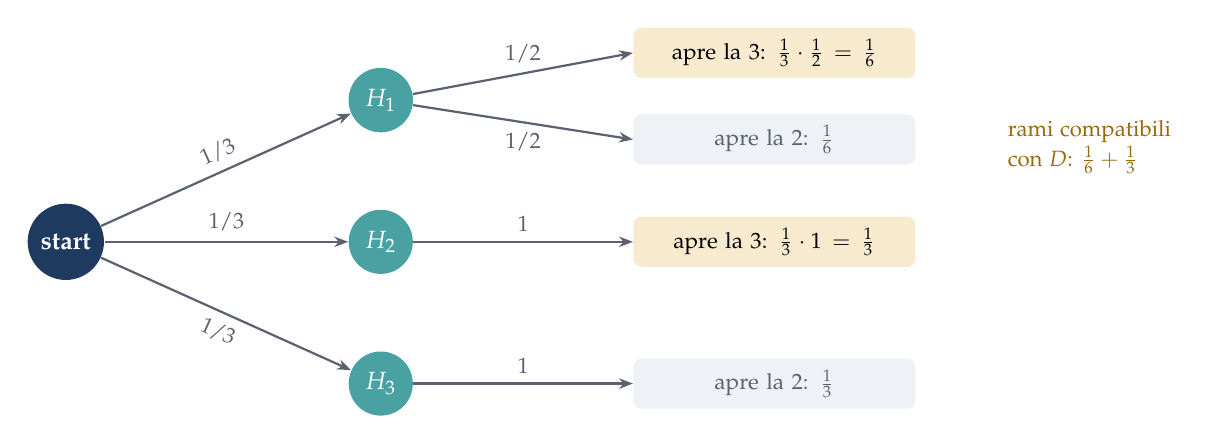
\begin{tikzpicture}[
  lev/.style={draw=none,font=\headfont\small},
  edge/.style={-{Stealth[length=5pt]},line width=.8pt,color=grigio},
  leaf/.style={rounded corners=3pt,font=\headfont\footnotesize,inner sep=4pt,text width=3.3cm,align=center},
  x=1cm,y=1cm]
\node[circle,fill=navy,text=white,font=\headfont\bfseries\small,minimum size=.9cm] (r) at (0,0) {start};
\node[circle,fill=teal!80,text=white,font=\headfont\small,minimum size=.8cm] (a) at (4,1.8) {$H_1$};
\node[circle,fill=teal!80,text=white,font=\headfont\small,minimum size=.8cm] (b) at (4,0) {$H_2$};
\node[circle,fill=teal!80,text=white,font=\headfont\small,minimum size=.8cm] (c) at (4,-1.8) {$H_3$};
\draw[edge] (r) -- node[above,sloped,font=\footnotesize]{1/3} (a);
\draw[edge] (r) -- node[above,font=\footnotesize]{1/3} (b);
\draw[edge] (r) -- node[below,sloped,font=\footnotesize]{1/3} (c);
\node[leaf,fill=ambra!20] (a1) at (9,2.4) {apre la 3: $\tfrac13\cdot\tfrac12=\tfrac16$};
\node[leaf,fill=chiaro,text=grigio] (a2) at (9,1.3) {apre la 2: $\tfrac16$};
\node[leaf,fill=ambra!20] (b1) at (9,0) {apre la 3: $\tfrac13\cdot1=\tfrac13$};
\node[leaf,fill=chiaro,text=grigio] (c1) at (9,-1.8) {apre la 2: $\tfrac13$};
\draw[edge] (a) -- node[above,font=\footnotesize]{1/2} (a1.west);
\draw[edge] (a) -- node[below,font=\footnotesize]{1/2} (a2.west);
\draw[edge] (b) -- node[above,font=\footnotesize]{1} (b1);
\draw[edge] (c) -- node[above,font=\footnotesize]{1} (c1);
\node[font=\headfont\footnotesize,text=ambra!70!black,align=left] at (13.0,1.2) {rami compatibili\\con $D$: $\tfrac16+\tfrac13$};
\end{tikzpicture}
\end{center}
\didascalia{Albero delle probabilità: tra i rami in cui il conduttore apre la 3 (evidenziati), quello con l'auto dietro la porta 2 pesa il doppio.}

\subsection{Perché l'intuizione sbaglia}
\begin{intuizione}
\begin{itemize}
  \item La tua scelta iniziale aveva probabilità $1/3$, e il conduttore non può cambiarla: qualunque cosa ci sia dietro la porta 1, lui una capra da mostrarti ce l'ha sempre. Quindi $P(H_1|D)$ resta $1/3$.
  \item Il conduttore \textbf{non apre a caso}: è vincolato a evitare l'auto. La sua scelta porta informazione, ed è proprio la likelihood asimmetrica ($1/2$ contro $1$) a spostare la probabilità sulla porta 2.
  \item Versione estrema: 100 porte, ne scegli una, il conduttore ne apre 98 con capre e ne lascia chiusa una sola. Terresti la tua (1/100) o cambieresti (99/100)?
\end{itemize}
\end{intuizione}
\begin{mlbox}[Il legame con la lezione]
È la stessa struttura del classificatore: \textbf{prior} (le porte equiprobabili), \textbf{likelihood} (quanto è probabile l'osservazione sotto ogni ipotesi), \textbf{evidence} (normalizzazione) e regola \textbf{MAP} (scegli l'ipotesi con posteriori massima: la porta 2). Bisogna modellare correttamente \emph{come sono stati generati i dati}: se il conduttore aprisse una porta a caso e per puro caso mostrasse una capra, le posteriori sarebbero davvero 1/2 e 1/2.
\end{mlbox}

\begin{appunti}{— Sezione 13}
\pag{62} Prior $1/3$ per porta. Likelihood che il conduttore apra la 3: $1/2$ ($H_1$), $1$ ($H_2$), $0$ ($H_3$). $P(D)=1/2$. Posteriori: porta 1 $=1/3$, porta 2 $=2/3$ → \textbf{conviene cambiare}. Il conduttore non agisce a caso: la sua scelta è informazione. Se aprisse a caso: 1/2 e 1/2.
\end{appunti}

\clearpage
\refstepcounter{section}
\addcontentsline{toc}{section}{\protect\numberline{}Formulario e anteprima}
\markboth{Formulario}{Formulario}

\begin{tikzpicture}
  \fill[navy,rounded corners=8pt] (0,0) rectangle (\textwidth,1.9cm);
  \node[anchor=west,font=\headfont\bfseries\fontsize{19}{23}\selectfont,text=white] at (.6cm,1.15cm) {Formulario riassuntivo};
  \node[anchor=west,font=\headlight\small,text=white!80!teal] at (.6cm,.45cm) {Le formule da sapere, in una pagina};
\end{tikzpicture}
\vspace{6pt}

\renewcommand{\arraystretch}{1.55}\small
\rowcolors{1}{white}{chiaro}
\begin{tabularx}{\linewidth}{>{\headfont\bfseries\small\color{navy}}m{3.5cm} >{\centering\arraybackslash}X}
Probabilità condizionata & $P(A|B)=\dfrac{P(A\cap B)}{P(B)}$ \qquad indipendenza: $P(A\cap B)=P(A)P(B)$\\
Probabilità totale & $p(\x)=\sum_{i=1}^{s}p(\x|w_i)P(w_i)$\\
Teorema di Bayes & $P(w_i|\x)=\dfrac{p(\x|w_i)\,P(w_i)}{p(\x)}$\\
Regola MAP & $b=\argmax_i P(w_i|\x)=\argmax_i\, p(\x|w_i)P(w_i)$\\
Probabilità di errore & $\displaystyle P(\mathrm{err})=\int_{\Re_1}p(x|w_2)P(w_2)\,dx+\int_{\Re_2}p(x|w_1)P(w_1)\,dx$\\
Stima a conteggio & $p(\x|w_i)\approx\dfrac{k_i}{n_i V}$ \qquad $P(w_i|\x)\approx\dfrac{k_i}{k}$\\
Normale 1D & $p(x)=\dfrac{1}{\sigma\sqrt{2\pi}}\,e^{-\frac{(x-\mu)^2}{2\sigma^2}}$\\
MLE 1D & $\hat\mu=\frac1n\sum_i x_i$ \qquad $\hat\sigma^2=\frac1n\sum_i(x_i-\hat\mu)^2$\\
Multinormale & $p(\x)=\dfrac{1}{(2\pi)^{d/2}|\SSigma|^{1/2}}\exp\!\big[-\tfrac12(\x-\mmu)\T\SSigma^{-1}(\x-\mmu)\big]$\\
MLE multivariata & $\mmu=\frac1n\sum_i\x_i$ \qquad $\SSigma=\frac1n\sum_i(\x_i-\mmu)(\x_i-\mmu)\T$\\
Mahalanobis & $r^2=(\x-\mmu)\T\SSigma^{-1}(\x-\mmu)$\\
Inversa $2\times2$ & $\left(\begin{smallmatrix}a&b\\c&d\end{smallmatrix}\right)^{-1}=\dfrac{1}{ad-bc}\left(\begin{smallmatrix}d&-b\\-c&a\end{smallmatrix}\right)$\\
Autovalori & $A\vv=\lambda\vv$ \qquad $\det(A-\lambda I)=0$ \qquad $\det A=\prod_k\lambda_k$\\
Discriminante & $g_i(\x)=-\frac12 r_i^2-\frac12\ln|\SSigma_i|+\ln P(w_i)$ \;(+ cost.)\\
N. parametri & $\mmu$: $d$ \qquad $\SSigma$: $\frac{d(d+1)}{2}$ \qquad Naive Bayes: $2d$\\
\end{tabularx}
\renewcommand{\arraystretch}{1.25}

\vspace{10pt}
\begin{tcolorbox}[base,colback=ambra!7,colbacktitle=ambra,coltitle=white,borderline west={3pt}{0pt}{ambra},title={Anteprima: approccio non parametrico (Parzen Window)},top=13pt]
Il sommario della lezione (slide 2 e 24) annuncia anche il metodo \textbf{Parzen Window}, che non è trattato in queste 62 slide. L'idea parte dalla formula della sezione 4, $p(\x)\approx k/(nV)$: invece di contare i punti in un cerchio fisso, si centra una piccola «finestra» (una funzione kernel, spesso gaussiana, di larghezza $h$) su \emph{ogni} campione del training set e si sommano i contributi:
\[
p(\x)\approx\frac1n\sum_{i=1}^{n}\frac{1}{h^d}\,\varphi\!\left(\frac{\x-\x_i}{h}\right)
\]
La larghezza $h$ regola il compromesso visto nella sezione 5: $h$ piccolo dà una stima piena di picchi (overfitting), $h$ grande una stima troppo liscia (underfitting).
\end{tcolorbox}

\vspace{4pt}
{\headfont\bfseries\color{navy}Per approfondire}
\begin{itemize}
  \item R. O. Duda, P. E. Hart, D. G. Stork, \emph{Pattern Classification}, 2ª ed., Wiley, 2001: capitolo 2 (teoria della decisione bayesiana) e capitolo 3 (stima MLE).
  \item K. Fukunaga, \emph{Introduction to Statistical Pattern Recognition}, Academic Press, 1990: test di normalità.
  \item S. Russell, P. Norvig, \emph{Artificial Intelligence: A Modern Approach}, 4ª ed., Pearson, 2021: capitolo sull'incertezza e gli assiomi della probabilità.
\end{itemize}

\end{document}
